\documentclass{article}
\usepackage[utf8]{inputenc}
\usepackage[english]{babel}
\usepackage{graphicx}
\usepackage{framed}
\usepackage[normalem]{ulem}
\usepackage{amsmath}
\usepackage{amsthm}
\usepackage{amssymb}
\usepackage{amsfonts}
\usepackage{enumerate}
\usepackage[utf8]{inputenc}
% \usepackage[top=1 in,bottom=1in, left=1 in, right=1 in]{geometry}
\usepackage{dsfont}
\usepackage{tikz}
\usepackage[unicode, colorlinks=true]{hyperref}
\usepackage{listings}
\usepackage[ruled,vlined]{algorithm2e}
\usepackage{extarrows}
\usetikzlibrary{patterns}
\usetikzlibrary{arrows}

\usepackage{graphicx}
\usepackage{caption}
\usepackage{subcaption}
\usepackage[section]{placeins}

\usepackage{amsmath}
\usepackage{mathtools}
\usepackage{dsfont}
\usepackage{amssymb}
\usepackage{amsthm}

% \usepackage{physics}
\usepackage{combelow}
\useshorthands{'}
\defineshorthand{'s}{\cb{s}}
\defineshorthand{'t}{\cb{t}}
\defineshorthand{'S}{\cb{S}}
\defineshorthand{'T}{\cb{T}}

\usepackage{enumitem}

\usepackage{stackengine}

\usepackage[super]{nth}

\usepackage[
backend=biber,
style=alphabetic,
sorting=ynt
]{biblatex}

\addbibresource{mybib.bib}

\usepackage{hyperref}
\hypersetup{
    colorlinks=true,
    linkcolor=blue,
    filecolor=magenta,      
    urlcolor=cyan,
}

\usepackage{graphicx,wrapfig,lipsum}

\lstset{
numbers=left, 
numberstyle=\small, 
numbersep=4pt, 
linewidth=10.5cm,
linewidth=16cm,
language=Python
}

\usepackage{tcolorbox}
\tcbuselibrary{listings, breakable, skins}

\newtcblisting{mylisting}{
  enhanced,
  breakable,
  listing only,
  sharp corners,
  arc=0mm,
  colback=white,
  boxsep=0mm,
  top=0mm,
  bottom=.6mm,
  left=7mm,
  right=1mm,
  boxrule=.7pt,
%   width=12.7cm,
  listing options={
    numbers=left,
    numberstyle=\small, 
    numbersep=8pt, 
    language=Python, 
    escapeinside={(*}{*)}
  }
}

%A bunch of definitions that make my life easier
\newcommand{\matlab}{{\sc Matlab} }
\newcommand{\cvec}[ 1]{{\mathbf #1}}
\newcommand{\rvec}[1]{\vec{\mathbf #1}}
\newcommand{\ihat}{\hat{\textbf{\i}}}
\newcommand{\jhat}{\hat{\textbf{\j}}}
\newcommand{\khat}{\hat{\textbf{k}}}
\newcommand{\minor}{{\rm minor}}
\newcommand{\trace}{{\rm trace}}
\newcommand{\spn}{{\rm Span}}
\newcommand{\rem}{{\rm rem}}
\newcommand{\ran}{{\rm range}}
\newcommand{\range}{{\rm range}}
\newcommand{\mdiv}{{\rm div}}
\newcommand{\proj}{{\rm proj}}
\newcommand{\R}{\mathbb{R}}
\newcommand{\N}{\mathbb{N}}
\newcommand{\Q}{\mathbb{Q}}
\newcommand{\Z}{\mathbb{Z}}
\newcommand{\<}{\langle}
\renewcommand{\>}{\rangle}
\renewcommand{\emptyset}{\varnothing}
\newcommand{\attn}[1]{\textbf{#1}}
\theoremstyle{definition}
\newtheorem{theorem}{Theorem}
\newtheorem{corollary}{Corollary}
\newtheorem*{definition}{Definition}
\newtheorem*{example}{Example}
\newtheorem*{note}{Note}
\newtheorem{exercise}{Exercise}
\newcommand{\bproof}{{\bf Proof. }}
\newcommand{\solution}{{\bf Solution. }}

\newcommand{\eproof}{\hfill\qedsymbol}
\newcommand{\Disp}{\displaystyle}
\newcommand{\qe}{\hfill\(\bigtriangledown\)}
\setlength{\columnseprule}{1 pt}

\usetikzlibrary{calc}

\def\gA{{\mathcal{A}}}
\def\gB{{\mathcal{B}}}
\def\gC{{\mathcal{C}}}
\def\gD{{\mathcal{D}}}
\def\gE{{\mathcal{E}}}
\def\gF{{\mathcal{F}}}
\def\gG{{\mathcal{G}}}
\def\gH{{\mathcal{H}}}
\def\gI{{\mathcal{I}}}
\def\gJ{{\mathcal{J}}}
\def\gK{{\mathcal{K}}}
\def\gL{{\mathcal{L}}}
\def\gM{{\mathcal{M}}}
\def\gN{{\mathcal{N}}}
\def\gO{{\mathcal{O}}}
\def\gP{{\mathcal{P}}}
\def\gQ{{\mathcal{Q}}}
\def\gR{{\mathcal{R}}}
\def\gS{{\mathcal{S}}}
\def\gT{{\mathcal{T}}}
\def\gU{{\mathcal{U}}}
\def\gV{{\mathcal{V}}}
\def\gW{{\mathcal{W}}}
\def\gX{{\mathcal{X}}}
\def\gY{{\mathcal{Y}}}
\def\gZ{{\mathcal{Z}}}

% Sets
\def\sA{{\mathbb{A}}}
\def\sB{{\mathbb{B}}}
\def\sC{{\mathbb{C}}}
\def\sD{{\mathbb{D}}}
% Don't use a set called E, because this would be the same as our symbol
% for expectation.
\def\sF{{\mathbb{F}}}
\def\sG{{\mathbb{G}}}
\def\sH{{\mathbb{H}}}
\def\sI{{\mathbb{I}}}
\def\sJ{{\mathbb{J}}}
\def\sK{{\mathbb{K}}}
\def\sL{{\mathbb{L}}}
\def\sM{{\mathbb{M}}}
\def\sN{{\mathbb{N}}}
\def\sO{{\mathbb{O}}}
\def\sP{{\mathbb{P}}}
\def\sQ{{\mathbb{Q}}}
\def\sR{{\mathbb{R}}}
\def\sS{{\mathbb{S}}}
\def\sT{{\mathbb{T}}}
\def\sU{{\mathbb{U}}}
\def\sV{{\mathbb{V}}}
\def\sW{{\mathbb{W}}}
\def\sX{{\mathbb{X}}}
\def\sY{{\mathbb{Y}}}
\def\sZ{{\mathbb{Z}}}

\def\sone{{\mathds{1}}}


\newcommand{\ld}{L_{\gD}}
\newcommand{\fd}{f_{\gD}}
\newcommand{\uset}{\underset}

\newcommand{\xyd}{(x, y) \in \gD}
\newcommand{\xysd}{(x, y) \sim \gD}
\newcommand{\ysdyx}{y \sim \gD_{y \mid x}}

\newcommand{\fxqy}{\fd(x) = y}
\newcommand{\fxny}{\fd(x) \neq y}
\newcommand{\gxny}{g(x) \neq y}

\newcommand{\ofxny}{\mathds{1}_{[\fxny]}}
\newcommand{\ogxny}{\mathds{1}_{\gxny}}

\newcommand{\exyd}{\uset{\xysd}{E}}
\newcommand{\exd}{\uset{x \sim \gD_x}{E}}
\newcommand{\exdyx}{\uset{x \sim \gD_{y \mid x}}{E}}

\newcommand{\oeless}{\sone_{[\eta(x) < \frac{1}{2}]}}
\newcommand{\oegeq}{\sone_{[\eta(x) \geq \frac{1}{2}]}}

\newcommand{\pydyx}{\uset{\ysdyx}{P}}

\newcommand{\hrs}{\gH_{rec}^2}
\newcommand{\hrd}{\gH_{rec}^d}
\newcommand{\hcd}{\gH_{con}^d}
\newcommand{\vcd}[1]{VC \dim{#1}}
\newcommand{\vchr}{\vcd(\hrd)}

\newcommand{\sft}[2]{\{#1, \dots, #2\}}
\newcommand{\szo}{\{0, 1\}}
\newcommand{\som}{\sft{1}{m}}

\newcommand{\izo}{(0, 1)}

\newcommand{\epd}{(\epsilon, \delta)}

\newcommand{\mgh}{m_{\gH}}

\newcommand{\psdm}{\uset{S \sim \gD^m}{P}}
\newcommand{\lfd}{L_{f, \gD}}

\newcommand{\ps}{P_S}
\newcommand{\psx}{P_S(x)}
\newcommand{\psxi}{P_S(x_i)}
\newcommand{\psxz}{P_S(x_0)}

\newcommand{\hs}{h_S}
\newcommand{\hsx}{h_S(x)}
\newcommand{\hsxi}{h_S(x_i)}
\newcommand{\hsxz}{h_S(x_0)}

\newcommand{\sRd}{\sR^d}
\newcommand{\sRs}{\sR^2}

% https://tex.stackexchange.com/questions/118173/
\DeclarePairedDelimiter\ceil{\lceil}{\rceil}
\DeclarePairedDelimiter\floor{\lfloor}{\rfloor}

\def\sone{{\mathds{1}}}


\newcommand{\ld}{L_{\gD}}
\newcommand{\fd}{f_{\gD}}
\newcommand{\uset}{\underset}
\newcommand{\usub}[2]{\underset{\substack{#1}}{#2}}

\newcommand{\xyd}{(x, y) \in \gD}
\newcommand{\xysd}{(x, y) \sim \gD}
\newcommand{\ysdyx}{y \sim \gD_{y \mid x}}

\newcommand{\fxqy}{\fd(x) = y}
\newcommand{\fxny}{\fd(x) \neq y}
\newcommand{\gxny}{g(x) \neq y}

\newcommand{\ofxny}{\mathds{1}_{[\fxny]}}
\newcommand{\ogxny}{\mathds{1}_{\gxny}}

\newcommand{\exyd}{\uset{\xysd}{E}}
\newcommand{\exd}{\uset{x \sim \gD_x}{E}}
\newcommand{\exdyx}{\uset{x \sim \gD_{y \mid x}}{E}}

\newcommand{\oeless}{\sone_{[\eta(x) < \frac{1}{2}]}}
\newcommand{\oegeq}{\sone_{[\eta(x) \geq \frac{1}{2}]}}

\newcommand{\pydyx}{\uset{\ysdyx}{P}}

\newcommand{\hin}{\gH_{\text{intervals}}}
\newcommand{\hro}{\gH_{rec}^1}
\newcommand{\hrs}{\gH_{rec}^2}
\newcommand{\hrd}{\gH_{rec}^d}
\newcommand{\hcd}{\gH_{con}^d}
\newcommand{\hmc}{\gH_{\text{mcon}}^d}
\newcommand{\hnp}{\gH_{\text{n-parity}}}
\newcommand{\hkx}[1]{\gH_{=#1}^{\gX}}
\newcommand{\ham}[1]{\gH_{\text{at-most-}#1}}

\newcommand{\vcd}[1]{\text{VCdim}(#1)}
\newcommand{\vchr}{\vcd{\hrd}}
\newcommand{\vch}{\vcd{\gH}}

\newcommand{\sft}[2]{\{#1, \dots, #2\}}
\newcommand{\szo}{\{0, 1\}}
\newcommand{\szod}{\{0, 1\}^d}
\newcommand{\szom}{\{0, 1\}^m}
\newcommand{\szon}{\{0, 1\}^n}
\newcommand{\som}{\sft{1}{m}}

\newcommand{\rft}[2]{#1, \dots, #2}

\newcommand{\izo}{(0, 1)}

\newcommand{\epd}{(\epsilon, \delta)}

\newcommand{\mgh}{m_{\gH}}

\newcommand{\pxsd}{\uset{x \sim \gD}{P}}
\newcommand{\psdm}{\uset{S \sim \gD^m}{P}}
\newcommand{\lfd}{L_{f, \gD}}

\newcommand{\loss}{\text{Loss}}

\newcommand{\ps}{P_S}
\newcommand{\psx}{P_S(x)}
\newcommand{\psxi}{P_S(x_i)}
\newcommand{\psxz}{P_S(x_0)}

\newcommand{\hs}{h_S}
\newcommand{\hsx}{h_S(x)}
\newcommand{\hsxi}{h_S(x_i)}
\newcommand{\hsxz}{h_S(x_0)}

\newcommand{\sRd}{\sR^d}
\newcommand{\sRs}{\sR^2}

\newcommand{\col}{\colon}
\newcommand{\ra}{\rightarrow}

\newcommand{\dt}{D^{(t)}}
\newcommand{\dti}{D^{(t)}(i)}
\newcommand{\dso}{D^{(1)}}
\newcommand{\doi}{D^{(1)}(i)}
\newcommand{\dtw}{D^{(2)}}
\newcommand{\dtwi}{D^{(2)}(i)}
\newcommand{\dtt}{D^{(t+1)}}
\newcommand{\dtti}{D^{(t+1)}(i)}

\newcommand{\bdt}{\mathbf{D}^{(t)}}
\newcommand{\bdti}{\mathbf{D}^{(t)}(i)}
\newcommand{\bdo}{\mathbf{D}^{(1)}}
\newcommand{\bdoi}{\mathbf{D}^{(1)}(i)}
\newcommand{\bdtt}{\mathbf{D}^{(t+1)}}
\newcommand{\bdtti}{\mathbf{D}^{(t+1)}(i)}

\newcommand{\zto}{Z_{t+1}}
\newcommand{\ztw}{Z_{2}}

\title{Machine Learning Theory \\ Exercise Handbook}
\author{Compiled by Matei Bejan \\ Faculty of Mathematics and Computer Science \\ University of Bucharest}
\date{August 2020}

\begin{document}

% \maketitle

\vspace*{\fill}
    \begin{center}
        \Huge{Statistical Learning Theory \\ Exercise Handbook}\\
        \vspace{1mm}
        \Large{Compiled by Matei Bejan \\ Faculty of Mathematics and Computer Science \\ University of Bucharest}\\
        \vspace{1mm}
        \large{February 2021}
    \end{center}
    \vspace*{\fill}

\newpage

\section*{Foreword}

\hspace{0.42cm} I wish for this work to be a statement. 

A statement against all the oppression, the mistreatment and the dehumanisation we've been subjected to for too long.

A statement against the abject labour we are forced into, that of desperately searching for a match and a light into a labyrinth of ever-growing darkness, being ever mislead by the very people we are expected to see as our tutors.

\vspace{1mm}

It is time all Computer Science students, regardless of gender, colour, religion or creed, to be united into one strong voice and, like thunder in a roaring tempest, to strike directly at the heart of those keeping us in the dark. 

For too long the authors of the great works of theoretical machine learning have forced us into such a grueling labour, to grind through their 1000-page tomes in order to find the one (or even two, if God  wills it!) exercises with solutions.

For too long the prestigious, prodigious professors have prophesied fruitless exercises that oft as not help build up little to no intuition and experience in solving the most frequent problems in this field.

For too long have we desperately begged Google for help, frantically searching for answers that the very prophets of this field keep away from our minds.

For too long have we been misguided, have we been deliberately stirred away from the knowledge, the information, the intuition we need to solve those types of exercises mentioned above.

\vspace{1mm}

The tyranny of darkness ends today. The age of intentional ignorance comes to a close. And is it we that shall send it to its binary grave!

Rise, fellow CompSci students, they fear us! 

They fear our intellect, so they stash away their prised solutions and give us convoluted proofs that are as helpful as jar of sand to a Saharan traveller!

They fear our ingenuity, so the few exercises we're being fed present all but little variation in topics!

They fear our adaptability, so they keep exaggerating the difficulty of their seminar work or book examples in order to confuse us!

\vspace{3mm}

Today, my friends, fear we shall give them! I speak to you all, oh students!, let your eyes feast on the exercises and solutions provided in this book and learn. Learn and show them once and for all that they cannot fool us into studying useless notions for our exams!

To those that have already pushed the boulders of Sisif and withstood the plight that are ML theory seminars, assignments and exams, I call thee to contribute to this work, to add more problems and solutions, more variation, more nuances of difficulty and even more sections!

\vspace{1mm}

An to you all, scornful professors and authors, those that deliberately keep us locked in the basement of our ignorance, you shall see us rise, learn and best you lot!

\vspace{3mm}

\hspace{9cm} The Compiler

\newpage

\section*{Contributors}

I would like to thank everyone who contributed to this work. If you've contributed via GitHub, please add your name (or at least your GitHub) to this list.

\begin{itemize}
    \item[] Marius Micul't\u{a}-C\^{a}mpeanu, University of Bucharest, Romania.
    \item[] 'Stefan Mereu't\u{a}, University of Bucharest, Romania.
    \item[] Andrei Manolache, University of Bucharest, Romania.
    \item[] Rob van Gastel,  Eindhoven University of Technology, Netherlands.
\end{itemize}

\newpage

\section*{Purpose}

The purpose of this hereby booklet is to centralize as many exercises and solutions to frequently asked exam and homework problems in the theoretical machine learning world. 
It is well known that computer science students usually lack formal, mathematical rigor, which they replace with what they call "common sense" or intuition. In order to help build that intuition, we've decided it would be best to create a central resource for problems, so that we can increase the sample size of the training data and thus help them achieve the best empirical loss.

Please do note that only a small portion of the solutions presented here are provided by myself. Most are provided either by contributors or by selecting solved problems over the internet or from well-known theory books, such as those of the Shais`s or Mohri`s. My work here was simply compiling them into one booklet, so that others waste not the time I have wasted looking over the internet for intuitive solutions.

At the time the first version of this book was written (February 2021), most of the exercises come through either the assignments presented by professor Bogdan Alexe, Ph.D. (Faculty of Mathematics and Computer Science, University of Bucharest) to his students or Shai Ben-David`s and Shai Shalev-Shwarz`s \textit{Understanding Machine Learning} and Alon Gonen`s solutions for their proposed exercises (note that I only took a few problems from there, which I considered to have the most intuitive solutions).

I did not consider it important to attribute the exercises and solutions to their respective providers, as the purpose of the booklet is not to help the contributors get acknowledged, but to help other computer science students study theoretical machine learning.

In the case the reader may have the resources and noble generosity to contribute, he may do so at the following GitHub address: \url{https://github.com/mateibejan14/stl-exercise-handbook}. Please do remember to update both the LaTe$\mathcal{X}$ code and PDF documents, as well as providing additional recourses such as images in case those are needed.

\hspace{8cm} The Compiler (again)

\newpage

\tableofcontents

\newpage

\section{PAC-learnability}

\textbf{Exercise 1.} An axis aligned rectangle classifier in the plane
is a classifier that assigns the value 1 to a point if and only if it is inside a certain rectangle. Formally, given real numbers $a_1 \leq b_1$, $a_2 \leq b_2$, define the classifier $h_{(a_1, b_1, a_2, b_2)}$ by:

$$h_{(a_1, b_1, a_2, b_2)}(x_1, x_2) = 
     \begin{cases}
       1, & a1 \leq x_1 \leq b_1 \text{ and } a_2 \leq x_2 \leq b_2 \\
       0, &\text{otherwise}
     \end{cases}$$

The class of axis-aligned rectangles in the plane is defined as:'

$$\mathcal{H}^2_{rec} = \{h_{(a_1, b_1, a_2, b_2)} \ | \ a_1 \leq b_1, a_2 \leq b_2\}.$$

\begin{itemize}
    \item[a)] Prove that the class of axis-aligned rectangles is PAC-learnable and show that the learning algorithm provided is polynomial is \textit{d}, $1/\epsilon$ and in $\log(1/\delta)$.
    \item[b)] Prove that the algorithm you provided at \textit{a)} has a sample complexity of $m_H(\epsilon, 1/\delta)$.
\end{itemize}

\textbf{Solution.}

a)

\begin{align*}
\hrs = \left\{
  \begin{array}{ll}
   h_{(a_1, b_1, a_2, b_2)} \colon \sRs \rightarrow \{0, 1\},
     a_1 \leq b_1 \text{ and } a_2 \leq b_2, \\
   h_{(a_1, b_1, a_2, b_2)}(x_1, x_2) = 
     \begin{cases}
       1, & a1 \leq x_1 \leq b_1 \text{ and } a_2 \leq x_2 \leq b_2 \\
       0, &\text{otherwise}
     \end{cases}
  \end{array}
        \right\}
\end{align*}
$\hrs$ is an infinite size hypothesis class, it is called the class of all axis aligned
rectangles in the plane. We want to prove that $\hrs$ is PAC-learnable.

\begin{proof}
From the definition of PAC-learnability, we know that $\gH=\hrs$ is PAC-learnable
if there exists a function $\mgh \colon (0, 1)^2 \rightarrow \sN$ and there exists
a learning algorithm $A$ with the following property: for every $\epsilon, \delta > 0$,
for every labelling function $f \in \hrs$ (realizability case), for every distribution
$\gD$ on $\sRs$ when we run the learning algorithm $A$ on a training set $S$ consisting of
$m \geq \mgh(\epsilon, \delta)$ examples sampled i.i.d.\ from $\gD$ and labeled by $f$,
the algorithm $A$ returns a hypothesis $\hs \in \gH$ such that, with probability at least
$1-\delta$ (over the choice of examples), the real risk of $\hs$ is smaller than $\epsilon$:
\begin{align*}
&\uset{S \sim {\gD}^m}{P} (L_{f, \gD}(\hs) \leq \epsilon) \geq 1-\delta
\text{ or otherwise said} \\
&\uset{S \sim {\gD}^m}{P} (L_{f, \gD}(\hs) > \epsilon) < \delta
\end{align*}

First, we need to find the algorithm $A$.

We are under the realizability assumption, so there exists a labelling function
$f \in \gH, f = h_{(a_1^*, b_1^*, a_2^*, b_2^*)}^*$ that labels the training data.

Consider the training set $S = \left\{(x_1, y_1), (x_2, y_2), \dots, (x_m, y_m)
                                 \; \; \vline \;
                                 \begin{array}{ll}
                                   y_i = h_{(a_1^*, b_1^*, a_2^*, b_2^*)}^*(x_i), \\
                                   x_i \in \sRs, x_i = (x_{i1}, x_{i2})
                                 \end{array}
                               \right\}$

\begin{figure}[h]
\begin{tikzpicture}
    %% define points
    \def\Ai{1.5};
    \def\Bi{7};
    \def\Aii{0.7};
    \def\Bii{4.35};
    
    %% axes
    \draw[->, thick] (-1,0) -- (8.5,0);
    \draw[->, thick] (0,-1) -- (0,5.5);
    
    %% rectangle
    \draw (\Ai,\Aii) rectangle (\Bi,\Bii);
    
    %% points on the axes
    \draw (\Ai,0.1) -- + (0,-0.2) node[below] {$a_1^*$};
    \draw (\Bi,0.1) -- + (0,-0.2) node[below] {$b_1^*$};
    \draw (0.1,\Aii) -- + (-0.2,0) node[left] {$a_2^*$};
    \draw (0.1,\Bii) -- + (-0.2,0) node[left] {$b_2^*$};
    
    %% dashed lines from points to rectangle
    \draw[dashed] (\Ai,0) -- (\Ai,\Aii);
    \draw[dashed] (\Bi,0) -- (\Bi,\Aii);
    \draw[dashed] (0,\Aii) -- (\Ai,\Aii);
    \draw[dashed] (0,\Bii) -- (\Ai,\Bii);
    
    %% pluses and minuses
    \draw (-1,2.8) node[scale=1.5] {$-$};
    \draw (1,2.35) node[scale=1.5] {$-$};
    \draw (4,0.35) node[scale=1.5] {$-$};
    \draw (8,3) node[scale=1.5] {$-$};
    \draw (4.5,5) node[scale=1.5] {$-$};
    
    \draw (2.75,3) node[scale=1.5] {$+$};
    \draw (3.5,1.5) node[scale=1.5] {$+$};
    \draw (4.5,2.5) node[scale=1.5] {$+$};
    \draw (5.5,3.25) node[scale=1.5] {$+$};
    
    %% other text
    \draw (-1.5,5) node[scale=1.25] {$\mathbb{R}^2$};
    \draw (\Bi,\Bii) + (-0.25,-0.25) node {$R^*$};
\end{tikzpicture}
\end{figure}

$h^*$ labels each point drawn from the rectangle
$R^* = [a_1^*, b_1^*] \times [a_2^*, b_2^*]$ with label 1, and all other points with label 0.
So we have $h_{(a_1^*, b_1^*, a_2^*, b_2^*)}^* = \sone_{R^*}$

Consider the following algorithm $A$, that takes as input the training set $S$
and outputs $\hs$.

$h_S = h_{(a_{1S}, b_{1S}, a_{2S}, b_{2S})}$, where
\begin{align*}
  a_{1S} &= \uset{\substack{i=\overline{1,m} \\ y_i=1}}{\min\ x_{i1}}
  &a_{2S} &= \uset{\substack{i=\overline{1,m} \\ y_i=1}}{\min\ x_{i2}} \\
  b_{1S} &= \uset{\substack{i=\overline{1,m} \\ y_i=1}}{\max\ x_{i1}}
  &b_{2S} &= \uset{\substack{i=\overline{1,m} \\ y_i=1}}{\max\ x_{i2}}
\end{align*}

If all $y_i = 0$, then all points $x_i$ have label 0, so there is no positive example.
In this case, choose $z = (z_1, z_2)$ a point that is not in the training set $S$ and
take $a_{1S} = b_{1S} = z_1,\, a_{2S} = b_{2S} = z_2$.

As in the \todo{?}\underline{indication},
$\hs = h_{(a_{1S}, b_{1S}, a_{2S}, b_{2S})} = \sone_{[a_{1S}, b_{1S}] \times [a_{2S}, b_{2S}]}$
is the indicator function of the tightest rectangle
$R_S = [a_{1S}, b_{1S}] \times [a_{2S}, b_{2S}]$ enclosing all positive examples.

By construction, $A$ is an ERM, meaning that $L_{h^*, \gD}(\hs) = 0,\, \hs$ doesn`t make
any errors on the training set $S$.

\begin{figure}[h]
\begin{tikzpicture}
    %% define points
    \def\Ai{1.5};
    \def\Bi{7};
    \def\Aii{0.7};
    \def\Bii{4.35};
    
    \def\Ais{2.75};
    \def\Bis{5.5};
    \def\Aiis{1.5};
    \def\Biis{3.25};
    
    %% axes
    \draw[->, thick] (-1,0) -- (8.5,0);
    \draw[->, thick] (0,-1) -- (0,5.5);
    
    %% rectangles
    \draw (\Ai,\Aii) rectangle (\Bi,\Bii);
    \draw[blue] (\Ais,\Aiis) rectangle (\Bis,\Biis);
    
    %% points on the axes
    \draw (\Ai,0.1) -- + (0,-0.2) node[below] {$a_1^*$};
    \draw (\Bi,0.1) -- + (0,-0.2) node[below] {$b_1^*$};
    \draw (0.1,\Aii) -- + (-0.2,0) node[left] {$a_2^*$};
    \draw (0.1,\Bii) -- + (-0.2,0) node[left] {$b_2^*$};
    
    \draw (\Ais,0.1) -- + (0,-0.2) node[below] {$a_{1S}$};
    \draw (\Bis,0.1) -- + (0,-0.2) node[below] {$b_{1S}$};
    \draw (0.1,\Aiis) -- + (-0.2,0) node[left] {$a_{2S}$};
    \draw (0.1,\Biis) -- + (-0.2,0) node[left] {$b_{2S}$};
    
    %% dashed lines from points to rectangles
    \draw[dashed] (\Ai,0) -- (\Ai,\Aii);
    \draw[dashed] (\Bi,0) -- (\Bi,\Aii);
    \draw[dashed] (0,\Aii) -- (\Ai,\Aii);
    \draw[dashed] (0,\Bii) -- (\Ai,\Bii);
    
    \draw[dashed,blue] (0,\Biis) -- (\Ais,\Biis);
    \draw[dashed,blue] (0,\Aiis) -- (\Ais,\Aiis);
    \draw[dashed,blue] (\Ais,0) -- (\Ais,\Aiis);
    \draw[dashed,blue] (\Bis,0) -- (\Bis,\Aiis);
    
    %% pluses and minuses
    \draw (-1,2.8) node[scale=1.5] {$-$};
    \draw (1,2.35) node[scale=1.5] {$-$};
    \draw (4,0.35) node[scale=1.5] {$-$};
    \draw (8,3) node[scale=1.5] {$-$};
    \draw (4.5,5) node[scale=1.5] {$-$};
    
    \draw (2.75,3) node[scale=1.5] {$+$};
    \draw (3.5,1.5) node[scale=1.5] {$+$};
    \draw (4.5,2.5) node[scale=1.5] {$+$};
    \draw (5.5,3.25) node[scale=1.5] {$+$};
    
    %% other text
    \draw (-1.5,5) node[scale=1.25] {$\mathbb{R}^2$};
    \draw (\Bi,\Bii) + (-0.25,-0.25) node {$R^*$};
    \draw (\Bis,\Biis) + (-0.25,-0.25) node {$R_S$};
    
    \draw[<-,thick,red] (\Bis,2.5) -- + (3.5,0) node[right,align=left,black] {this is the rectangle $R_S$ \\ \underline{implemented}(?) by \\ $h_{(a_{1S}, b_{1S}, a_{2S}, b_{2S})}$};
\end{tikzpicture}
\end{figure}

Now we want to find the sample complexity $\mgh\epd$ such that
\begin{equation*}
\uset{S \sim {\gD}^m}{P} (L_{h^*, \gD}(\hs) \leq \epsilon) \geq 1-\delta \text{ where } S
\text{ contains } m \geq \mgh\epd \text{ examples.}
\end{equation*}

We make the observation that $\hs$ can make errors in region $R^* \setminus R_S$, labelling
points that should get label 1 with label 0. All points $\in R$\footnote{$R_S$?} will be labeled correctly,
all points outside $R^*$ will be labeled correctly.

Let`s fix $\epsilon > 0, \delta > 0$ and consider a distribution $\gD$ over $\sRs$.

\begin{enumerate}[itemindent=0.5cm,label=Case \arabic*)]
  \item
  \begin{align*}
    \text{If }\gD(R^*) =& \uset{x \sim \gD}{P}(x \in R^*) \leq \epsilon
      \text{ then in this case} \\
    L_{h^*, \gD}(\hs)  =& \uset{x \sim \gD}{P}(\hsx \neq h^*(x)) =
      \uset{x \sim \gD}{P}(x \in R^* \setminus R_S) \leq
      \uset{x \sim \gD}{P}(x \in R^*) \leq \epsilon \text{ so we have that} \\
    &\psdm(L_{h^*, \gD}(\hs) \leq \epsilon) = 1
      \text{ (this happens all the time)}
  \end{align*}

  \item $\gD(R^*) = \uset{x \sim \gD}{P}(x \in R^*) > \epsilon$
    
    \begin{figure}[h]
    \begin{tikzpicture}
        %% define points
        \def\Ai{1.5};
        \def\Bi{7};
        \def\Aii{0.7};
        \def\Bii{4.35};
        
        \def\Ais{2.75};
        \def\Bis{5.5};
        \def\Aiis{1.5};
        \def\Biis{3.25};
        
        \def\Ri{2.15};
        \def\Rii{6.2};
        \def\Riii{1.2};
        \def\Riv{3.75};
        
        %% axes
        \draw[->, thick] (-1,0) -- (8.5,0);
        \draw[->, thick] (0,-1) -- (0,5.5);
        
        %% rectangles
        \draw (\Ai,\Aii) rectangle (\Bi,\Bii);
        \draw[blue] (\Ais,\Aiis) rectangle (\Bis,\Biis);
        
        %% points on the axes
        \draw (\Ai,0.1) -- + (0,-0.2) node[below] {$a_1^*$};
        \draw (\Bi,0.1) -- + (0,-0.2) node[below] {$b_1^*$};
        \draw (0.1,\Aii) -- + (-0.2,0) node[left] {$a_2^*$};
        \draw (0.1,\Bii) -- + (-0.2,0) node[left] {$b_2^*$};
        
        \draw (\Ais,0.1) -- + (0,-0.2) node[below] {$a_{1S}$};
        \draw (\Bis,0.1) -- + (0,-0.2) node[below] {$b_{1S}$};
        \draw (0.1,\Aiis) -- + (-0.2,0) node[left] {$a_{2S}$};
        \draw (0.1,\Biis) -- + (-0.2,0) node[left] {$b_{2S}$};
        
        \draw (\Ri,0.1) -- + (0,-0.2) node[below] {$a_1$};
        \draw (\Rii,0.1) -- + (0,-0.2) node[below] {$b_1$};
        \draw (0.1,\Riii) -- + (-0.2,0) node[left] {$a_2$};
        \draw (0.1,\Riv) -- + (-0.2,0) node[left] {$b_2$};
        
        %% dashed lines from points to rectangles
        \draw[dashed] (\Ai,0) -- (\Ai,\Aii);
        \draw[dashed] (\Bi,0) -- (\Bi,\Aii);
        \draw[dashed] (0,\Aii) -- (\Ai,\Aii);
        \draw[dashed] (0,\Bii) -- (\Ai,\Bii);
        
        \draw[dashed,blue] (0,\Biis) -- (\Ais,\Biis);
        \draw[dashed,blue] (0,\Aiis) -- (\Ais,\Aiis);
        \draw[dashed,blue] (\Ais,0) -- (\Ais,\Aiis);
        \draw[dashed,blue] (\Bis,0) -- (\Bis,\Aiis);
        
        \draw[dashed,red] (0,\Riv) -- (\Ai,\Riv);
        \draw[dashed,red] (0,\Riii) -- (\Ai,\Riii);
        \draw[dashed,red] (\Ri,0) -- (\Ri,\Aii);
        \draw[dashed,red] (\Rii,0) -- (\Rii,\Aii);
        
        %% R1, R2, R3, R4
        \draw[red] (\Ri,\Aii) -- (\Ri,\Bii) node[midway,left,black] {R1};
        \draw[red] (\Rii,\Aii) -- (\Rii,\Bii) node[midway,right,black] {R2};
        \draw[red] (\Ai,\Riii) -- (\Bi,\Riii) node[midway,below,black] {R3};
        \draw[red] (\Ai,\Riv) -- (\Bi,\Riv) node[midway,above,black] {R4};
        
        %% pluses and minuses
        \draw (-1,2.8) node[scale=1.5] {$-$};
        \draw (1,2.35) node[scale=1.5] {$-$};
        \draw (4,0.35) node[scale=1.5] {$-$};
        \draw (8,3) node[scale=1.5] {$-$};
        \draw (4.5,5) node[scale=1.5] {$-$};
        
        \draw (2.75,3) node[scale=1.5] {$+$};
        \draw (3.5,1.5) node[scale=1.5] {$+$};
        \draw (4.5,2.5) node[scale=1.5] {$+$};
        \draw (5.5,3.25) node[scale=1.5] {$+$};
        
        %% other text
        \draw (-1.5,5) node[scale=1.25] {$\mathbb{R}^2$};
        \draw (\Bi,\Bii) + (-0.25,-0.25) node {$R^*$};
        \draw (\Bis,\Biis) + (-0.25,-0.25) node {$R_S$};
    \end{tikzpicture}
    \end{figure}
\end{enumerate}
We construct as in the indication the 4 rectangles $R_1, R_2, R_3, R_4$:
\begin{align*}
  &\begin{array}{l}
    R_1 = [a_1^*, a_1] \times [a_2^*, b_2^*] \qquad
    R_2 = [b_1, b_1^*] \times [a_2^*, b_2^*] \\
    R_3 = [a_1^*, b_1^*] \times [a_2^*, a_2] \qquad
    R_4 = [a_1^*, b_1^*] \times [b_2, b_2^*] 
  \end{array}
  \qquad
  \text{with } \gD(R_i) = \uset{x \sim \gD}{P}(x \in R_i) = \frac{\epsilon}{4}
\end{align*}
% https://tex.stackexchange.com/questions/460561/
If $R$\footnote{$R_S$?} $= [a_{1S}, b_{1S}] \times [a_{2S}, b_{2S}]$
(the rectangle returned by $A$, implemented by $\hs$)
intersects each $R_i, i=\overline{1, 4}$:
\begin{align*}
  L_{h^*, \gD}(\hs) &=
    \uset{x \sim \gD}{P}(h^*(x) \neq \hsx) =
    \uset{x \sim \gD}{P}(x \in R^* \setminus R_S) \leq
    \uset{x \sim \gD}{P}(x \in R_1 \cup R_2 \cup R_3 \cup R_4) \leq \\
   &\leq \sum_{i=1}^4 \uset{x \sim \gD}{P}(x \in R_i)
       = \sum_{i=1}^4 \gD(R_i) = 4 \cdot \frac{\epsilon}{4} = \epsilon
\end{align*}

So, in this case,
$\psdm(L_{h^*, \gD}(\hs) \leq \epsilon) = 1$ (this happens always).

In order to have $L_{h^*, \gD}(\hs) > \epsilon$, we need that $R_S$ will not intersect
at least one rectangle $R_i$.

We denote with $F_i = \{S \sim \gD^m \mid R_S \cap R_i = \emptyset\}$.
This leads to the following:
\begin{align*}
  \psdm(L_{h^*, \gD}(\hs) > \epsilon) = 
  \psdm(\overbracket[0pt][0pt]{
    F1 \cup F2 \cup F3 \cup F4)
  \leq}^{
      \substack{\text{at least one } F_i \text{ will happen} \\ \quad\nearrow\hfill\phantom{.}
      }} \sum_{i=1}^4 \psdm(F_i)
\end{align*}

\begin{flalign*}
  \text{Now, } \psdm(F_i) &=
      \text{ what is the probability that $R_S$ will not intersect } R_i & \\
  & = \text{ the probability that no point from $R_i$ is sampled in } S & \\
  & = \left(1-\frac{\epsilon}{4}\right)^m &
\end{flalign*}
So \[
\psdm(L_{h^*, \gD}(\hs) > \epsilon) \leq
  \sum_{i=1}^4\psdm(F_i) = 4 \cdot \left(1 - \frac{\epsilon}{4}\right)^m
\]
Now, we know from lecture 2 that $1-x \leq e^{-x}$,
so $1-\frac{\epsilon}{4} \leq e^{-\frac{\epsilon}{4}}$, which means that
\[
\psdm\uset{\substack{\qquad\quad\uparrow\hfill\phantom{.} \\
\text{this is the probability to have}\\ \text{ $\hs$ will make(??) error } > \,\epsilon}}{(
  L_{h^*, \gD}(\hs) > \epsilon)} \leq
4 \cdot \left(1 - \frac{\epsilon}{4}\right)^m \leq 4 \cdot e^{-\frac{\epsilon}{4} m}
\]
We want to make this probability very small, smaller than $\delta$:
\begin{align*}
  4 \cdot e^{-\frac{\epsilon}{4} m} &< \delta \\
  e^{-\frac{\epsilon}{4} m} &< \left. \frac{\delta}{4}
    \quad \right\lvert \cdot \log_e \\
  -\frac{\epsilon}{4} \cdot m &< \log\frac{\delta}{4}
    \; \left\lvert \cdot \left(-\frac{4}{\epsilon}\right) \right. \\
  m &> -\frac{4}{\epsilon} \log \frac{\delta}{4} = \frac{4}{\epsilon} \log \frac{4}{\delta}
\end{align*}
So, if we take $m \geq \mgh\epd = \frac{4}{\epsilon}\cdot\log\frac{4}{\delta}$,
we obtain the desired results.

\vspace{0.2cm}

\noindent Repeat the previous question for the class of aligned rectangles in $\sRd$.

\noindent In $\sRd$, we have
\begin{align*}
  \hrd = \left\{
  \begin{array}{rl}
    &h_{(a_1, b_1, a_2, b_2, \dots, a_d, b_d)} \colon \sRd \rightarrow \szo \mid a_i \leq b_i, i = \overline{1, d} \\
    &h_{(a_1, b_1, a_2, b_2, \dots, a_d, b_d)} =
  \sone_{[a_1, b_1] \times [a_2, b_2] \times \dots \times [a_d, b_d]}
  \end{array}  
  \right\}
\end{align*}
All the arguments used previously will work, the general result will be that
$\mgh\epd = \frac{2d}{\epsilon} \cdot \log \frac{2d}{\delta}$.

\noindent For $d = 2$, we obtain the previous result.

The runtime of algorithm $A$ is given by taking \todo{?} \underline{minimum}\footnote{min,max?} over each dimension, so this means $\gO(m*d)$: $m = $ number of (positive) examples
$ = \gO(\frac{2d}{\epsilon} \cdot \log \frac{2d}{\delta})$ \\
$d = $ number of dimensions.

So we have that the complexity of algorithm $A$ is $\gO(\frac{2d^2}{\epsilon} \cdot \log \frac{2d}{\delta})$, which is polynomial in $d$, $\frac{1}{\epsilon}$, $\frac{1}{\delta}$.

\end{proof}

b) 

\begin{enumerate}[label=\alph*)]
%   \item \label{prop:a} Given $\delta \in \izo$ and given $0 < \epsilon_1 \leq \epsilon_2 < 1$, we have that
%     $\mgh(\epsilon_1, \delta) \geq \mgh(\epsilon_2, \delta)$.

\begin{proof}
$\gH$ is PAC-learnable with sample complexity $\mgh(\cdot, \cdot)$ means that there exists
a learning algorithm $A$ with the following property: for every $\epsilon, \delta > 0$, when
we run the algorithm $A$ on a sample set $S$ of $m$ examples, $m \geq \mgh\epd$
(samples are labeled by $f \in \gH$ and i.i.d.\ from a distribution $\gD$), we have that
$\hs = A(S)$ with the real risk $\psdm(\lfd(\hs) \leq \epsilon) > 1-\delta$.

We apply this for $\epsilon_1$ and $\delta$:
\[\psdm(\lfd(\hs) \leq \epsilon_1) > 1-\delta
\text{ if } m \geq \mgh(\epsilon_1, \delta)\]

We know that $\epsilon_2 \geq \epsilon_1$, so we have that
\[\psdm(\lfd(\hs) \leq \epsilon_2) > 1-\delta \text{ if } m \geq \mgh(\epsilon_1, \delta)\]

But $\mgh(\epsilon_2, \delta)$ is the smallest number of examples for which the above inequality
holds. So, if it holds for $m \geq \mgh(\epsilon_1, \delta)$, we have that
$\mgh(\epsilon_1, \delta) \geq \mgh(\epsilon_2, \delta)$.
\end{proof}

  \item Given $\epsilon \in \izo$, $0 < \delta_1 \leq \delta_2 < 1$, we have that
  $\mgh(\epsilon, \delta_1) \geq \mgh(\epsilon, \delta_2)$.
  \begin{proof}
  Using the same arguments from \ref{prop:a}, we have that
  \begin{align*}
    \psdm(\lfd(\hs) \leq \epsilon) > 1-\delta_1 \text{ if } m \geq \mgh(\epsilon, \delta_1) \\
    \delta_1 \leq \delta_2 \Rightarrow 1-\delta_1 \geq 1-\delta_2 \Rightarrow 
    \psdm(\lfd(\hs) \leq \epsilon) > 1-\delta_2 \text{ if } m \geq \mgh(\epsilon, \delta_1)
  \end{align*}
  
  But $\mgh(\epsilon, \delta_2)$ is the smallest number of examples for which the above
  inequality holds\\(if ${m \geq \mgh(\epsilon, \delta_2)}$). So, if it holds for
  $m \geq \mgh(\epsilon, \delta_1)$, we have that
  $\mgh(\epsilon, \delta_1) \geq \mgh(\epsilon, \delta_2)$.
  \end{proof}
\end{enumerate}

\textbf{Exercise 2.} Consider H to be the class of all centered in origin sphere classifiers in the 3D space. A centered in origin sphere classifier in the 3D space is a classifier $h_r$ that assigns the value 1 to a point if and only if it is inside the sphere with radius $r > 0$ and center given by the origin O(0,0,0). Consider the realizability assumption. 

Show that H can be $(\epsilon, \delta)-PAC$ learned by giving an algorithm A and determining the sample complexity $m_H (\epsilon, \delta)$ such that the definition of PAC-learnability is satisfied.

\textbf{Solution.}

The classifiers described in the problem are formally closed center-origin balls in $\mathbb{R}^3$. We can rewrite H as follows:

$$H = \{ B[0, r] | r \in \mathbb{R}_{+}\} \subset \mathbb{R}^3$$

Let A be the following algorithm:

\begin{mylisting}
if (*$\exists s \in S \subset \mathbb{R}^2 \times \{\text{label } | \text{ label } \in \{0,1\} \}$*) with label 1:
    (*$r = \underset{\text{label(s) = 1} }{\max ||s||}$*)
else:
    (*$r = \underset{\text{label(s) = 0}}{\min ||s||} - 10^{-1000} $*)
return B[0, r]
\end{mylisting}

In other words, our algorithm A returns the minimal-volume sphere that contains all 1-labelled samples. In case no such samples exist, we return the sphere with the diameter smaller than the closest 0-labeled point to the origin.

We denote with $h_A, r_A$ the hypothesis returned by our algorithm and its associated radius, respectively. By assuming realizability, we denote with $h^*$ the hypothesis with zero error and with $r^*$, its radius. 

Let $\epsilon, \delta \in (0,1)$ and $r' \in \mathbb{R}, r' \leq r^*$, such that $D[{x|r' \leq ||x|| \leq r^*}] = \epsilon$. Next, let $E=B[0, r^*] \setminus B[0, r']$ represent the error area between our classifier and the zero-error classifier. 

% maybe use $$ 
$\underset{S \sim D^{m}}{P}[L_D(h_S) \geq \epsilon] < P[\not\exists x|x \in S \setminus E] < (1 - \epsilon^m) < e^{-\epsilon m}$

We want $e^{-\epsilon m} < \delta \Rightarrow m > \frac{\log \delta}{\epsilon}$. 
%m_{H} (\epsilon, \delta) < \lceil \frac{\log \delta^{-1}}{\epsilon} \rceil$.

\begin{figure}[hbt!]
\centering
\begin{tikzpicture}[scale=.79]
\shade[ball color = green!40, opacity = 0.3] (0,0) circle (2cm);
\shade[ball color = red!20, opacity = 0.8] (0,0) circle (1cm);
\draw (0,0) circle (2cm);
\draw[dotted] (-2,0) arc (180:360:2 and 0.6);
\draw[dotted] (2,0) arc (0:180:2 and 0.6);
\fill[fill=black] (0,0) circle (1pt);
\draw[dashed] (0,0 )--(2,0);
\node (p1) at (1.5,1.5) [label={$h^*$}]{};
\node (p2) at (.2,.2) [label={$h_A$}]{};
\node (p3) at (.9,.9) [label={$E$}]{};
\end{tikzpicture}
% \caption{on of error area $E$.}
\label{fig:my_label}
\end{figure}

\textbf{Exercise 3.} Let X be a discrete domain, and let $H_{Singleton} = {h_z | z \in \chi } \cup {h^- }$, where for each $z \in \chi$ , $h_z$ is the function defined by $h_z (x) = 1$ if x = z and $h_z (x) = 0$ if $x \neq z$. $h ^-$ is simply the all-negative hypothesis, namely, $\forall x \in X, h^- (x) = 0$.
The realizability assumption here implies that the true hypothesis f labels negatively all examples in the domain, perhaps except one.

\begin{itemize}
    \item[a.] Describe an algorithm that implements the ERM rule for learning $H_{Singleton}$ in the realizable setup.
    \item[b.] Show that $H_{Singleton}$ is PAC learnable. Provide an upper bound on the sample complexity.
\end{itemize}

\textbf{Solution.} 

$\gX$ discrete domain, $\gH_\text{Singleton} = \{h_z \colon z \in \gX\} \cup \{h^-\}$
\begin{align*}
  &\forall z \in \gX \quad
    h_z \colon \gX \rightarrow \szo, \quad
    h_z(x) = \begin{cases}
      1, & x = z \\
      0, & x \neq z
    \end{cases} \\
  &h^- \colon \gX \rightarrow \szo, \quad h^-(x) = 0, \; \forall x \in \gX
\end{align*}
\subparagraph{a)} Describe an algorithm that implements the ERM rule for learning
$\gH_\text{Singleton}$ in the realizable setup.
\begin{proof}

\noindent Consider
$S = \{(x_i, h^*(x_i)),\, x_i \text{ i.i.d.\ from a distribution $\gD$ over } \gX\}_{i=1}^m$.

\noindent The algorithm $A$ is the following:

\indent Loop over training examples \\
\indent   If there is an $i \in \som$ such that $y_i = 1$, then
            return hypothesis $\hs = A(S) = h_{x_i}$ \\
\indent   Otherwise return $h^-$.

From construction, $A$ is ERM, meaning that $L_S(\hs) = 0$.
\end{proof}
\subparagraph{b)} Show that $\gH_\text{Singleton}$ is PAC-learnable. Provide an upper bound on the sample complexity.
\begin{proof}
Let $\epsilon, \delta > 0$ and fix a distribution $\gD$ over $\gX$.

\noindent The only case in which the algorithm $A$ fails is the case where $h^* = h_z$ and the
sample\\
$S = \{(x_i, y_i) \mid $ \todo{?} $x_i$ sampled i.i.d.\ from $\gD\}$ doesn`t contain any positive
examples, so all $y_i = 0 \; \forall i = \overline{1, m}$.

\noindent In this case, $\hs = A(S) = h^-$, which is different from $h^*$. However, even if the
algorithm $A$ fails if $\gD(\{z\}) \leq \epsilon$, then everything is ok, as we have that:
\[ \psdm(L_{h^*, \gD}(\hs) \leq \epsilon) = 1 \quad \checkmark\checkmark \]

\noindent So, we have to upper bound the sample complexity in the case where
$\gD(\{z\}) > \epsilon$ and there is no positive example in the set $S$ (actually, for
this problem, there is just one positive possible training point $= z$).
We have that
\begin{flalign*}
&\psdm(L_{h^*, \gD}(\hs) > \epsilon) = \text{probability that each point in } S &\\
  &\text{ is different than } z \:
 (\text{which has probability mass} > \epsilon) \leq (1-\epsilon)^m \leq e^{-\epsilon m}& \\
&\text{So, if we set }
  e^{-\epsilon m} < \delta \Rightarrow -\epsilon m < \log \delta &\\
&\qquad m > -\frac{1}{\epsilon} \log \delta \Rightarrow m > \frac{1}{\epsilon} \log \frac{1}{\delta} &\\
&\text{If } m \geq \left\lceil \frac{1}{\epsilon} \log \frac{1}{\delta} \right\rceil
\text{we have that } \psdm(L_{h^*, \gD}(\hs) > \epsilon) < \delta &\\
&\text{So the upper bound of } \mgh\epd \text{ is } \mgh\epd \leq
\left\lceil \frac{1}{\epsilon} \log \frac{1}{\delta} \right\rceil &
\end{flalign*}
\end{proof}

\textbf{Exercise 4.} An axis aligned square classifier in the plane is a classifier that assigns the value 1 to a point if and only if it is inside a certain square. Formally, given the real numbers $a_1, a_2, r> 0\in\mathbb{R}$ we define the classifier $h_{(a_1, a_2, r)}$ by.

\begin{equation}
h_{a_1, a_2, r}(x_1, x_2) = 
\begin{cases}
    1 & a_1 \leq x_1 \leq a_1 + r, a_2 \leq x_2 \leq a_2 + r \\
    0 & \text{otherwise} \\
\end{cases}
\end{equation}

the class of all axis aligned squares in the plane is defined as

$$\mathcal{H}=\{h_{a_1, a_2, r}:\mathbb{R}^2\to\{0,1\}|a_1, a_2, r\in \mathbb{R}, r>0\}$$

Consider the realizability assumption.

a) Give a learning algorithm $\mathcal{A}$ that returns a hypothesis $h_S=\mathcal{A}(S)$ that has empirical risk 0 on $S$.

b) Find the sample complexity $m_\mathcal{H}(\varepsilon, \delta)$ in order to show that $\mathcal{H}$ is PAC-learnable.

\textbf{Solution.}

a) Consider the following ERM algorithm $\mathcal{A}$: Let $S_p$ be the set of all positive labeled points in the sample $S$. Project all the points in $S_p$ on the $Ox$ axis and let $S_{px}$ be the set of scalars obtained by taking the $x$ component of the projection, pick $a_1^* = min(\{S_{px}\})$ and $r_x=max(\{S_{px}\})$, do the same on the $Oy$ axis and build the $S_{py}$ set, pick $a_2^*=min(\{S_{py}\})$ and $r_y=max(\{S_{py}\})$. Let $r^*=max(\{||a_1^*-r_x||_2, ||a_2^*-r_y||_2\})$, pick the hypothesis $h_{a_1^*, a_2^*, r^*}$, which is the square that most "tightly" contains all the positive examples, so it is correctly labeling them. 

If the obtained square has 0-labeled points from $S$ inside it, translate it on the $Ox$ and $Oy$ directions until there is no 0-labeled point inside - the realizability assumption guarantees that there exists a square $\Tilde{R}$ corresponding to the real labeling function that perfectly labels all the points, so for our minimum enclosing square, we'll either eventually get a square that`s included in $\Tilde{R}$, so it is ERM, or a square that is just partially included in $\Tilde{R}$ but it still is ERM (since it has no more negative points from the training set inside). 

b) The proof is very similar to the axis-aligned rectangles problem. Let $R(x,y,z,h)$ be the rectangle as defined in the axis aligned rectangles problem and $R(x,y,z)$ be a the rectangle $R(x, x+z, y, y+z)$.

Fix a distribution $\mathcal{D}$ over $\mathcal{X}$ and let $h_{\Tilde{a_1}, \Tilde{a_2}, \Tilde{r}}=\Tilde{h}$ be the hypothesis with 0 generalization error and $R(\Tilde{a_1}, \Tilde{a_2}, \Tilde{r}) = \Tilde{R}$ the associated square. Let $R(S)$ be the square returned by the ERM algorithm $\mathcal{A}$ for the training sequence $S$.

Let $\varepsilon, \delta \in (0, 1)$, and let $a_{12}>\Tilde{a_1}$ such that $R_1=R(\Tilde{a_1}, a_{12}, \Tilde{a_2}, \Tilde{a_2}+\Tilde{r})$ has probability mass $\frac{\varepsilon}{8}$ w.r.t. the distribution $\mathcal{D}$. In a similar fashion, get 3 more rectangles $R_2 = R(a_{11}, \Tilde{a_1}+\Tilde{r}, \Tilde{a_2}, \Tilde{a_2}+\Tilde{r}), R_3 = R(\Tilde{a_1}, \Tilde{a_1}+\Tilde{r}, a_{21}, \Tilde{a_2}+\Tilde{r}), R_4 = R(\Tilde{a_1}, \Tilde{a_1}+\Tilde{r}, \Tilde{a_2}, a_{22})$ such that every one of them has mass $\frac{\varepsilon}{8}$. 

Until now, the reasoning was identical to that of the axis-aligned rectangles (except for the probability mass of $\frac{\epsilon}{8}$). Now construct one more square as below:

\begin{figure}
    \centering

        \begin{tikzpicture}
        \draw[step=1cm,gray,very thin] (-1.9,-1.9) grid (9.9,3.9);
        \filldraw[blue!40!white, draw=black] (0,-1) rectangle (4,3);
        \filldraw[red!40!white, draw=black] (4,-1) rectangle (8,3);
        
        \filldraw[yellow!40!white, draw=black, opacity=0.5] (1,-1.5) rectangle (4,1.5);
        
        % \node at (2,-1.5){$\Tilde{R}$};
        % \node at (6,-1.5){$SQ$};
        
        \node at (3.5,2){$\frac{\varepsilon}{8}$};

        \node at (4.5,2){$\frac{\varepsilon}{8}$};

        \draw[dashed] (3, 3) -- (3, -1);
        \draw[dashed] (5, 3) -- (5, -1);

        \end{tikzpicture}

  \caption{Blue: the optimal square $\Tilde{R}$; Red: the square $SQ$ - same area as $\Tilde{R}$; Transparent yellow: $\mathcal{A}(S)$, the errors from landing below $\Tilde{R}$ are taken into account by the way $SQ$ is constructed.}
  \label{fig:drawing}
\end{figure}

The square $SQ$ in the right has the same mass as the optimal square $\Tilde{R}$. Construct 4 more rectangles $R_5 \dots R_{8}$ with probability mass $\frac{\varepsilon}{8}$ w.r.t. $\mathcal{D}$ on $SQ$ the same way we did on $\Tilde{R}$. 

We don`t care about the other 7 squares (on the diagonals, in the left or the ones on top and bottom), we take into account possible errors from them on $SQ$ since we're assuming realizability and the total area of the square returned from $\mathcal{A}$ can be at most as big as that of $\Tilde{R}$, and the biggest error appears if $\mathcal{A}$ returns one of the squares like $SQ$ (if it sees just 2 corner points on one border of $\Tilde{R}$).

We have that $\mathcal{L}_{(\mathcal{D}, \Tilde{h})}(R(S))=\mathcal{D}((\Tilde{R} \backslash R(S)) \cup (R(S) \cap SQ))$.


Now, for $\forall i \in \overline{1,8}$ define $F_i=\{S|_x | S|_x \cap R_i = \emptyset \}$; for a sequence of $m$ points we have that 

\begin{equation}
    \mathcal{D}^m(\{ S | \mathcal{L}_{(\mathcal{D}, \Tilde{h})}(\mathcal{A}(S)) > \varepsilon \}) \leq \mathcal{D}^m(\underset{i \in \overline{1,8} }{\bigcup}F_i)
\end{equation}

By applying Boole`s inequality we get that

\begin{equation}
    \mathcal{D}^m(\underset{i \in \overline{1,8} }{\bigcup}F_i) \leq \underset{i \in \overline{1,8}}{\sum}\mathcal{D}^m(F_i)
\end{equation}

Now take an arbitrary, but fixed $i \in \overline{1,8}$ - if we have a sample in $F_i$ we know that there`s some sample that is not in $R_i$, so $\mathcal{D}^m(F_i) = (1 - \frac{\varepsilon}{8})^m \leq e^{-m\frac{\varepsilon}{8}}$. Combining $(2)$ and $(3)$ we get that

\begin{equation}
    \mathcal{D}(\{ S | \mathcal{L}_{(\mathcal{D}, \Tilde{h})}(\mathcal{A}(S)) > \varepsilon \}) \leq 
    8e^{-m\frac{\varepsilon}{8}}
\end{equation}

Now we can see that as our sample size grows, the probability to have errors gets smaller, pick $\delta \geq 8e^{-m\frac{\varepsilon}{8}}$, we compute that $-m\frac{\varepsilon}{8}\leq log(\frac{\delta}{8}) \Rightarrow -m \leq \frac{8}{\varepsilon}log(\frac{\delta}{8}) \Rightarrow m \geq \frac{8}{{\varepsilon}}log(\frac{8}{\delta})$.

\vspace{3mm}

\textbf{Exercise 5 .} An axis aligned square classifier in the plane is a classifier that assigns the value 1 to a point if and only if it is inside a certain square. Formally, given the real numbers $a_1, a_2, r > 0 \in \sR$ we define the classifier $h_{(a_1, a_2, r)}$ by
\[
h_{(a_1, a_2, r)}(x_1, x_2) = 
\begin{cases}
  1 & \text{if } a_1 \leq x_1 \leq a_1+r, a_2 \leq x_2 \leq a_2+r \\
  0 & \text{otherwise}
\end{cases}
\]
The class of all axis-aligned squares in the plane is defined as
\[\gH = \{h_{(a_1, a_2, r)} \col \sR^2 \ra \szo \mid a_1, a_2, r \in \sR,\; r > 0\}\]
Consider the realizability assumption.
\begin{enumerate}[label=\textbf{\alph*.},ref=\alph*)]
\item \label{4:a} give a learning algorithm $A$ that returns a hypothesis $h_S$ from
$\gH$, $h_S = A(S)$ consistent with the training set $S$ ($h_S$ has empirical risk 0 on $S$);
\item\label{4:b} find the sample complexity $m_{\gH}\epd$ in order to show that $\gH$ is
PAC-learnable;
\item\label{4:c} compute $\vch$.
\end{enumerate}

\textbf{Solution}.

\begin{proof}

Consider the realizability assumption: there $\exists \: h_{(a_1^*, a_2^*, r^*)}$
labeling the training data.

a) $S = \{(x_1, y_1), \dots, (x_i, y_i), \dots, (x_m, y_m)\}$,
$y_i = h_{(a_1^*, a_2^*, r^*)}(x_i)$.

We need to find $a_{1S}, a_{2S}, r_{S}$ such that
$\hs = A(S) = h_{a_{1S}, a_{2S}, r_{S}}$ is ERM.

\fbox{Sketch of proof}

\underline{Particular cases:} two positive or just 1 positive point in $S$.

\underline{General case:} more than 2 positive points in $S \rightarrow$
find the smallest rectangle containing all positive points. We need to extend
this rectangle such that we obtain a square.

\begin{tikzpicture}
    \draw (0,0) rectangle (3,3);
    \draw[blue] (1.5,1) rectangle (2.5,2.5);
    
    \draw (-0.5,2) node {$-$};
    \draw (1.5,-0.5) node {$-$};
    \draw (4,1.5) node {$-$};
    \draw (2.5,3.5) node {$-$};
    
    \draw (1.5,2.5) node {$+$};
    \draw (2.5,2) node {$+$};
    \draw (2,1) node {$+$};
    
    \draw (3.25,3.25) node {$R^*$};
    
    \draw (6,0) rectangle (9,3);
    \draw[blue] (6.5,1.5) rectangle (8.5,2.5);
    
    \draw (5.5,2) node {$-$};
    \draw (7.5,-0.5) node {$-$};
    \draw (10,1.5) node {$-$};
    \draw (8.5,3.5) node {$-$};
    
    \draw (6.5,2.5) node {$+$};
    \draw (8.5,2) node {$+$};
    \draw (7.5,1.5) node {$+$};
    
    \draw (9.25,3.25) node {$R^*$};
\end{tikzpicture}

Parameterize the rectangle by center $(x_0, y_0)$, width $w$, height $h$.
\begin{itemize}[label=-]
\item if $w = h$ \quad OK (we have a square)
\item without loss of generality, we can consider $h \geq w$.
\end{itemize}

\begin{tikzpicture}
    \draw (0,0) rectangle (3,3);
    \draw[blue] (1,0.5) rectangle (2,2.5);
    \draw[blue,dashed] (0.5,0.5) rectangle (2.5,2.5);
    
    \draw (-0.5,2) node {$-$};
    \draw (1.5,-0.5) node {$-$};
    \draw (4,1.5) node {$-$};
    \draw (2.5,3.5) node {$-$};
    
    \draw (1,2.5) node {$+$};
    \draw (2,2) node {$+$};
    \draw (1.5,0.5) node {$+$};
    
    \draw(1.5,1.5) node{$\cdot$};
    
    \draw (3.25,3.25) node {$R^*$};
    \draw (2.7,2.3) node {$R$};
    
    \draw (6,0) rectangle (9,3);
    \draw[blue] (7.75,0.5) rectangle (8.75,2.5);
    \draw[blue,dashed] (7.25,0.5) rectangle (9.25,2.5);
    
    \draw (5.5,2) node {$-$};
    \draw (7.5,-0.5) node {$-$};
    \draw (10,1.5) node {$-$};
    \draw (8.5,3.5) node {$-$};
    
    \draw (7.75,2.5) node {$+$};
    \draw (8.75,2) node {$+$};
    \draw (8.25,0.5) node {$+$};
    
    \draw (8.25,1.5) node{$\cdot$};
    
    \draw (9.25,3.25) node {$R^*$};
    \draw (9.45,2.3) node {$R$};
    
    \draw (10.25,1.5) node[align=left,right] {(could extend the initial \\ rectangle to a square \\ outside $R^*$)};
\end{tikzpicture}

Use the following steps:
\begin{enumerate}
  \item check if the square with center $(x_0, y_0)$ and side $= h$ contains a negative
    point. If not, return this square.
  \item If the previous constructed square contains negative points from $S$, then:
  \begin{itemize}[label=-]
    \item find $x_{\text{left}} =$ the largest value on the \nth{1} coordinate of a
      negative point in the left part of our rectangle; if $x_{\text{left}}$ does not
      exist, OK \checkmark $\ra$ we can build the square to the left
    \item find $x_{\text{right}} =$ the smallest value on the \nth{1} coordinate of a
      negative point in the right part of our initial rectangle; if there is no such
      negative point, OK $\Rightarrow$ we can build our desired square in the right
  \end{itemize}
\end{enumerate}

\begin{minipage}{0.51\textwidth}
\begin{tikzpicture}
    \draw[->] (-1,0) -- (7,0);
    \draw[->] (0,-1) -- (0,5);

    \draw (1.5,1) rectangle (4.5,4);
    \draw[blue] (3.3,1.5) rectangle (4.3,3.5);
    % \draw[blue,dashed] (2.8,1.5) rectangle (4.8,3.5);
    \draw[blue,dashed] (3.3,1.5) -- (2.8,1.5) -- (2.8,3.5) -- (3.3,3.5);
    \draw[blue,dashed] (4.3,1.5) -- (4.8,1.5) -- (4.8,3.5) -- (4.3,3.5);
    
    \draw (0.5,2.5) node {$-$};
    \draw (0.7,3.5) node {$-$};
    \draw (0.3,0.9) node {$-$};
    \draw (1,1.3) node {$-$};
    \draw (2.2,0.5) node {$-$};
    \draw (3,4.6) node {$-$};
    \draw (5,2.5) node {$-$};
    \draw (5.7,3.5) node {$-$};
    \draw (5.3,0.9) node {$-$};
    \draw (6,1.5) node {$-$};
    
    \draw (3.3,3.5) node {$+$};
    \draw (4.3,3) node {$+$};
    \draw (3.8,1.5) node {$+$};
    \draw (3.5,2) node {$+$};
    \draw (4.1,2.5) node {$+$};
    
    \draw[dashed] (1,0) -- (1,1.3) node[at start,below] {$x_\text{left}$};
    \draw[dashed] (5,0) -- (5,2.5) node[at start,below] {$x_\text{right}$};
    \draw[dashed] (0,1.5) -- (2.8,1.5) node[at start,left] {$a_2$};
    
    \draw(3.8,2.5) node{$\cdot$};
    
    \draw (4.75,4.25) node {$R^*$};
    \draw (5,3.2) node {$R$};
\end{tikzpicture}
\end{minipage}
\begin{minipage}{0.4\textwidth}
We do know that \boxed{x_{\text{right}} - x_{\text{left}} > h}

Take $\epsilon = \dfrac{x_{\text{right}} - x_{\text{left}} - h}{2} > 0$.

Then we can fit a square of side $h$ in
$[x_{\text{left}} + \epsilon, x_{\text{right}} - \epsilon] \times [a_2, a_2+h]$
(various ways to do this)
\end{minipage}

\phantom{.}

b) Two types of errors:
\begin{itemize}[label=-]
  \item false negatives in $R^* \setminus R$
  \begin{tikzpicture}
      \draw (0,0) rectangle (1.5,1.5);
      \draw (0.3,0.3) rectangle (1.2,1.2);
      
      \pattern[pattern=north west lines] (0,0) -- (0,1.5) -- (0.3,1.5) -- (0.3,0);
      \pattern[pattern=north west lines] (0.3,0) -- (0.3,0.3) -- (1.2,0.3) -- (1.2,0);
      \pattern[pattern=north west lines] (0.3,1.2) -- (0.3,1.5) -- (1.2,1.5) -- (1.2,1.2);
      \pattern[pattern=north west lines] (1.2,0) -- (1.2,1.5) -- (1.5,1.5) -- (1.5,0);
      
      \draw (0.5,0.8) node {$+$};
      \draw (0.75,1) node {$+$};
      \draw (1,0.6) node {$+$};
      
      \draw (-0.3,1) node {$-$};
      \draw (1,1.8) node {$-$};
      \draw (2,0.8) node {$-$};
      
      \draw[red] (0.3,1.35) node {$-$};
      
      \draw (1.75,1.4) node[scale=0.75] {$R^*$};
      \draw (1,1) node[scale=0.75] {$R$};
  \end{tikzpicture}
  \item false positives in $R \setminus R^*$
  \begin{tikzpicture}
      \draw (0,0) rectangle (1.5,1.5);
      \draw (0.9,0.3) rectangle (1.8,1.2);
      
      \pattern[pattern=north west lines] (1.5,0.3) -- (1.5,1.2) -- (1.8,1.2) -- (1.8,0.3);
      
      \draw (1,0.6) node {$+$};
      \draw (1.35,0.8) node {$+$};
      \draw (1.6,0.6) node[red] {$+$};
      
      \draw (-0.3,1) node {$-$};
      \draw (0.8,1.8) node {$-$};
      \draw (2,0.8) node {$-$};
      
      \draw (1.4,1.7) node[scale=0.75] {$R^*$};
      \draw (1.05,1) node[scale=0.75] {$R$};
  \end{tikzpicture}
\end{itemize}

Let $\epsilon > 0,\, \delta > 0$ and $\gD$ a probability distribution on $\sRs$.

Consider regions of probability mass $= \frac{\epsilon}{8}$.

\phantom{.}

\begin{minipage}{0.3\textwidth}
\begin{tikzpicture}
    \draw (0,0) rectangle (3,3);
    \draw (-0.5,0) rectangle (3.5,3);
    \draw (0,-0.5) rectangle (3,3.5);
    
    \draw (0,2.5) -- (3,2.5);
    \draw (0,0.5) -- (3,0.5);
    \draw (0.5,0) -- (0.5,3);
    \draw (2.5,0) -- (2.5,3);
    
    \draw (0.25,1.5) node {$R_1$};
    \draw (1.5,0.25) node {$R_2$};
    \draw (2.75,1.5) node {$R_3$};
    \draw (1.5,2.75) node {$R_4$};
    \draw (-0.25,1.5) node {$R_5$};
    \draw (1.5,-0.25) node {$R_6$};
    \draw (3.25,1.5) node {$R_7$};
    \draw (1.5,3.25) node {$R_8$};
\end{tikzpicture}
\end{minipage}
\begin{minipage}{0.5\textwidth}
\begin{align*}
L_{\text{FN}, i}(\hs) &= \pxsd[x \in R_i] \qquad i = \overline{1, 4} \\
L_{\text{FP}, i}(\hs) &= \pxsd[x \in R_{i+4}] \quad i = \overline{1, 4}
\end{align*}
\end{minipage}

\phantom{.}

So, if we want that $L_{\gD, h^*}(\hs) > \epsilon$, then one of the eight losses
$\geq \frac{1}{8}$.

\begin{align*}
\text{Define } F_i &= \left\{S \sim \gD^m \mid L_{\text{FN}, i}(\hs) \geq \frac{1}{8} \right\}
\quad i = \overline{1, 4} \\
F_{i+4} &= \left\{S \sim \gD^m \mid L_{\text{FP}, i}(\hs) \geq \frac{1}{8} \right\}
\quad i = \overline{1, 4}
\end{align*}
\begin{align*}
\text{So } &\psdm(L_{\gD, h^*}(\hs) > \epsilon) \leq \psdm(F_1 \cup \dots \cup F_8) \leq
  \sum_{i=1}^8 P(F_i) = 8 \cdot \left(1- \frac{\epsilon}{8} \right)^m \leq
  8 \cdot e^{-m \cdot \frac{\epsilon}{8}} < \delta \\
  &\Rightarrow \boxed{m > \frac{8}{\epsilon} \log \frac{8}{\delta}}
\end{align*} 

\end{proof}

\textbf{Exercise 6.} Give a PAC-learning algorithm for the concept class $\mathcal{C}$ formed by closed intervals [a,b] with $a, b \in \mathbb{R}$.

\vspace{1mm}

\textbf{Solution.}

\begin{align*}
\gC = \gH_\text{intervals}
    = \left\lbrace
      \begin{array}{ll}      
        h_{a, b} \colon \sR \rightarrow \{0, 1\}, a \leq b \\
        h_{a, b}(x) = \sone_{[a, b]}(x) = \left\lbrace
          \begin{array}{ll}
            1, x \in [a, b] \\
            0, \text{otherwise}
          \end{array}
          \right.
      \end{array}
    \right\rbrace
\end{align*}

Consider a training set $S = \{(x_1, y_1), (x_2, y_2), \dots, (x_m, y_m)\}$.
We are in the realizability case, ${\exists h^* = h_{a^*, b^*} \in \gH_\text{intervals}}$
that labels the examples, $y_i = h^*(x_i)$.

\begin{figure}[h]
\centering
\begin{tikzpicture}
    \draw[->] (0,0) -- (10,0);
    
    \draw (3,0.1) -- + (0,-0.2) node[below] {\mathstrut$a^*$};
    \draw (7,0.1) -- + (0,-0.2) node[below] {\mathstrut$b^*$};
    \draw (3.5,0.1) -- + (0,-0.2) node[below] {\mathstrut$a_S$};
    \draw (6.5,0.1) -- + (0,-0.2) node[below] {\mathstrut$b_S$};
    
    \draw (3.5,-0.1) -- + (0,0.2) node[above] {$+$};
    \draw (4.5,-0.1) -- + (0,0.2) node[above] {$+$};
    \draw (5.2,-0.1) -- + (0,0.2) node[above] {$+$};
    \draw (6.5,-0.1) -- + (0,0.2) node[above] {$+$};
    
    \draw (0.5,-0.1) -- + (0,0.2) node[above] {$-$};
    \draw (1.9,-0.1) -- + (0,0.2) node[above] {$-$};
    \draw (2.5,-0.1) -- + (0,0.2) node[above] {$-$};
    \draw (7.6,-0.1) -- + (0,0.2) node[above] {$-$};
    \draw (8.3,-0.1) -- + (0,0.2) node[above] {$-$};
    \draw (9.6,-0.1) -- + (0,0.2) node[above] {$-$};
\end{tikzpicture}
\end{figure}

We want to show that $\gH_\text{intervals}$ is PAC-learnable.

Consider $A$ the learning algorithm that gets the training set $S$ and outputs $h_S = A(S) = $ the tightest
interval containing all the positive examples.

\begin{align*}
  h_S = h_{a_S, b_S} \qquad \text{where} &&
  a_S = \uset{(x_i, 1) \in S}{\min x_i} &&
  b_S = \uset{(x_i, 1) \in S}{\max x_i} &&
  R_S = [a_S, b_S]
\end{align*}

If there is no $(x_i, 1) \notin S$ ($S$ doesn`t contain positive examples), take %% ???
$a_S = b_S = z$ a random point such that $(z, 0) \notin S$.

From construction, we see that $L_S(h_S) = 0$.

Let $\epsilon > 0, \delta > 0$ and $\gD$ a distribution over $R$.
How many training examples $m \geq m_{\gH}(\epsilon, \delta)$ do we need such that
\begin{equation*}
  \uset{S \sim \gD^m}{P}(L_{\gD, h^*}(h_S) > \epsilon) < \delta
\end{equation*}

Case 1: if $\gD([a^*, b^*]) \leq \epsilon$ then
  $\uset{S \sim \gD^m}{P}(L_{\gD, h^*}(h_S) > \epsilon) = 0$ \checkmark


Case 2: if $\gD([a^*, b^*]) > \epsilon$

Build $R_1$ and $R_2$, $R_1 = [a_1^*, a_1]$, $R_2 = [b_1, b_1^*]$ such that 
$\gD(R_1) = \gD(R_2) = \frac{\epsilon}{2}$.

\begin{figure}[h]
\centering
\begin{tikzpicture}
    \draw[->] (0,0) -- (5,0);
    \draw (1,0.1) -- + (0,-0.2) node[below] {\mathstrut$a_1^*$};
    \draw (4,0.1) -- + (0,-0.2) node[below] {\mathstrut$b_1^*$};
    \draw (1.5,0.1) -- + (0,-0.2) node[below] {\mathstrut$a_1$};
    \draw (3.5,0.1) -- + (0,-0.2) node[below] {\mathstrut$b_1$};
    
    \draw[decoration=brace,decorate] (1,0.15) -- (1.5,0.15) node[midway,above] {$\frac{\epsilon}{2}$ mass};
    \draw[decoration=brace,decorate] (3.5,0.15) -- (4,0.15) node[midway,above] {$\frac{\epsilon}{2}$ mass};
\end{tikzpicture}
\end{figure}

If $R_S \cap R_1 \neq \emptyset$ and $R_S \cap R_2 \neq \emptyset$ then
  $\uset{S \sim \gD^m}{P}(L_{\gD, h^*}(h_S) > \epsilon) = 0$ \checkmark

Else $\uset{S \sim \gD^m}{P}(L_{\gD, h^*}(h_S) > \epsilon)
        \leq 2 \cdot \left(1 - \frac{\epsilon}{2}\right)^m
        \leq 2 \cdot e^{-\frac{\epsilon}{2}m}
        < \delta
        \Rightarrow \boxed{m > \frac{2}{\epsilon} \log \frac{2}{\delta}}$

\vspace{3mm}

\textbf{Exercise 7.} Give a PAC-learning algorithm for the concept class $\mathcal{C}_2$ formed by unions of two closed intervals, that is $[a, b] \cup [c, d]$, with $a, b, c, d \in \mathbb{R}$. Extend your result to derive a PAC-learning algorithm for the concept class $\mathcal{C}_p$ formed by unions of $p \geq 1$ closed intervals, thus $[a_1, b_1] \cup \dots \cup [a_p, b_p]$, with $a_k, b_k \in \mathbb{R}, \forall k \in [p]$. What are the time and sample complexities of your algorithm as a function of p?

\vspace{1mm}

\textbf{Solution.}

PAC-learning algorithm for the class $\gC_2$ formed by unions of two closed intervals: 
\begin{align*}
  \gC_2 = \left\lbrace
    \begin{array}{ll}
      h_{(a, b, c, d)} \colon \sR \rightarrow [0, 1], \;
      h_{(a, b, c, d)} = \sone_{[a, b] \cup [c, d]} \\
      a \leq b \leq c \leq d, \;
      h_{(a, b, c, d)}(x) = \left\lbrace
        \begin{array}{ll}
          1, x \in [a, b] \cup [c, d] \\
          0, \text{otherwise}
        \end{array}
      \right.
    \end{array}
  \right\rbrace
\end{align*}

Consider $S = \{(x_1, y_1), (x_2, y_2), \dots, (x_m, y_m)\}$, where ${y_i = h^*(x_i), h^* = h_{(a^*, b^*, c^*, d^*)}}$ \footnote{realizability assumption}.

\begin{figure}[h]
\centering
\begin{tikzpicture}
    \draw[->] (0,0) -- (10,0);
    
    \draw (2,0) node {$[$} node[below=4] {$a^*$};
    \draw (4,0) node {$]$} node[below=4] {$b^*$};
    \draw (6,0) node {$[$} node[below=4] {$c^*$};
    \draw (8,0) node {$]$} node[below=4] {$d^*$};
    
    \draw (2.5,-0.1) -- + (0,0.2) node[above] {$+$};
    \draw (2.85,-0.1) -- + (0,0.2) node[above] {$+$};
    \draw (3.5,-0.1) -- + (0,0.2) node[above] {$+$};
    \draw (6.5,-0.1) -- + (0,0.2) node[above] {$+$};
    \draw (6.95,-0.1) -- + (0,0.2) node[above] {$+$};
    \draw (7.6,-0.1) -- + (0,0.2) node[above] {$+$};
    
    \draw (0.5,-0.1) -- + (0,0.2) node[above] {$-$};
    \draw (1.3,-0.1) -- + (0,0.2) node[above] {$-$};
    \draw (4.5,-0.1) -- + (0,0.2) node[above] {$-$};
    \draw (5.2,-0.1) -- + (0,0.2) node[above] {$-$};
    \draw (8.6,-0.1) -- + (0,0.2) node[above] {$-$};
    \draw (9.6,-0.1) -- + (0,0.2) node[above] {$-$};
\end{tikzpicture}
\end{figure}

Consider the following learning algorithm $A$ that takes input $S$:
\begin{enumerate}[label=\roman*)]
  \item Sort $S$ in ascending order of $x_i$
  \item Go over the sorted training examples and take the intervals where consecutive training
        examples labeled as positive start and end the intervals.
        You can obtain one or two intervals. In the case that there are no positive examples take $a_S = b_S = c_S = d_S = z$, where $z$ a random points such that $(z,0)$ doesn`t appear in the training set $S$.
  \item If you obtained just one interval, you can have
    $a_S = \uset{\uset{y_i = 1}{(x_i, y_i)}}{\min x_i}$,  %% y_i = -1 ???
    $b_S = \uset{\uset{y_i = 1}{(x_i, y_i)}}{\max x_i}$,
    $c_S = d_S = b_S$
    
    If you obtained two intervals, then
    $a_S = \uset{\uset{y_i = 1}{(x_i, y_i)}}{\min x_i}$,
    $d_S = \uset{\uset{y_i = 1}{(x_i, y_i)}}{\max x_i}$,
    $a_S \leq b_S < c_S \leq d_S$
    
    Return $h_S = h_{(a_S, b_S, c_S, d_S)} = \sone_{[a_S, b_S] \cup [c_S, d_S]}$.
\end{enumerate}
We need to find $m \geq m_{\gC_2}(\epsilon, \delta)$ such that for $\epsilon > 0$, $\delta > 0$
and for every $\gD$ distribution over $\sR$ we have
\begin{equation*}
  \uset{S \sim \gD^m}{P}(L_{\gD, h^*}(h_S) > \epsilon) < \delta
\end{equation*}
Let $\epsilon > 0$, $\delta > 0$ and let $\gD$ be a distribution over $\sR$.
 
The region where $h_S$ can make errors is always $\subseteq \; [a^*, d^*]$.
    
\underline{Case 1}: If $\gD([a^*, d^*]) \leq \epsilon$, then
  $\uset{S \sim \gD^m}{P}(L_{\gD, h^*}(h_S) > \epsilon) = 0$.

\underline{Case 2}: If $\gD([a^*, d^*]) > \epsilon$
  
The types of error that $h_S$ can make are:
\begin{itemize}[label=-]
  \item false negatives in $[a^*, b^*]$ and $[c^*, d^*]$
    \begin{figure}[h]
    \centering
    \begin{tikzpicture}
        \draw[->] (0,0) -- (10,0);
        
        \draw (1.5,0) node {$[$} node[below=4] {\mathstrut$a^*$};
        \draw (4.5,0) node {$]$} node[below=4] {\mathstrut$b^*$};
        \draw (5.5,0) node {$[$} node[below=4] {\mathstrut$c^*$};
        \draw (8.5,0) node {$]$} node[below=4] {\mathstrut$d^*$};
        
        \draw (2,0) node {$[$} node[below=4] {\mathstrut$a_S$};
        \draw (4,0) node {$]$} node[below=4] {\mathstrut$b_S$};
        \draw (6,0) node {$[$} node[below=4] {\mathstrut$c_S$};
        \draw (8,0) node {$]$} node[below=4] {\mathstrut$d_S$};
        
        \draw (2.85,-0.1) -- + (0,0.2) node[above] {$+$};
        \draw (3.5,-0.1) -- + (0,0.2) node[above] {$+$};
        \draw (6.5,-0.1) -- + (0,0.2) node[above] {$+$};
        \draw (6.95,-0.1) -- + (0,0.2) node[above] {$+$};
        \draw (7.6,-0.1) -- + (0,0.2) node[above] {$+$};
        
        \draw (0.5,-0.1) -- + (0,0.2) node[above] {$-$};
        \draw (1.1,-0.1) -- + (0,0.2) node[above] {$-$};
        \draw (5.1,-0.1) -- + (0,0.2) node[above] {$-$};
        \draw (8.8,-0.1) -- + (0,0.2) node[above] {$-$};
        \draw (9.6,-0.1) -- + (0,0.2) node[above] {$-$};
        
        \draw[decoration=brace,decorate] (1.5,0.25) -- (2,0.25) node[midway,above=2,scale=0.8] {error};
        \draw[decoration=brace,decorate] (4,0.25) -- (4.5,0.25) node[midway,above=2,scale=0.8] {error};
        \draw[decoration=brace,decorate] (5.5,0.25) -- (6,0.25) node[midway,above=2,scale=0.8] {error};
        \draw[decoration=brace,decorate] (8,0.25) -- (8.5,0.25) node[midway,above=2,scale=0.8] {error};
    \end{tikzpicture}
    \end{figure}
    
  \item false positive in $(b^*, c^*)$ if sample $S$ does not contain any points sampled from
    $(b^*, c^*)$.
    \begin{figure}[h]
    \centering
    \begin{tikzpicture}
        \draw[->] (0,0) -- (10,0);
        
        \draw (1.5,0) node {$[$} node[below=4] {\mathstrut$a^*$};
        \draw (4.5,0) node {$($} node[below=4] {\mathstrut$b^*$};
        \draw (5.5,0) node {$)$} node[below=4] {\mathstrut$c^*$};
        \draw (8.5,0) node {$]$} node[below=4] {\mathstrut$d^*$};
        
        \draw (2,0) node {$[$} node[below=4] {\mathstrut$a_S$};
        \draw (8,0) node {$]$} node[below=4] {\mathstrut$d_S$};
        
        \draw (2.85,-0.1) -- + (0,0.2) node[above] {$+$};
        \draw (3.5,-0.1) -- + (0,0.2) node[above] {$+$};
        \draw (6.5,-0.1) -- + (0,0.2) node[above] {$+$};
        \draw (6.95,-0.1) -- + (0,0.2) node[above] {$+$};
        \draw (7.6,-0.1) -- + (0,0.2) node[above] {$+$};
        
        \draw (0.5,-0.1) -- + (0,0.2) node[above] {$-$};
        \draw (1.1,-0.1) -- + (0,0.2) node[above] {$-$};
        \draw (8.8,-0.1) -- + (0,0.2) node[above] {$-$};
        \draw (9.6,-0.1) -- + (0,0.2) node[above] {$-$};
        
        \draw[decoration=brace,decorate] (1.5,0.25) -- (2,0.25) node[midway,above=2,scale=0.8] {error};
        \draw[decoration=brace,decorate] (4.5,0.25) -- (5.5,0.25) node[midway,above=2,scale=0.8] {error};
        \draw[decoration=brace,decorate] (8,0.25) -- (8.5,0.25) node[midway,above=2,scale=0.8] {error};
    \end{tikzpicture}
    \end{figure}
\end{itemize}
Denote $L_{FP}$, $L_{FN, 1}$, $L_{FN, 2}$ these type of errors, where:
\begin{align*}
  L_{FP}(h_S)
    &= \uset{x \sim \gD}{P}(
        x \in [a_S, b_S] \cup [c_S, d_S] \setminus
             ([a^*, b^*] \cup [c^*, d^*])
      ) \\
    &= \uset{x \sim \gD}{P}(x \in [b^*, c^*] \subseteq [a_S, b_S] \cup [c_S, d_S]) \\
  L_{FN, 1}(h_S)
    &= \uset{x \sim \gD}{P}(x \in [a^*, b^*] \setminus [a_S, b_S]) \\
  L_{FN, 2}(h_S)
    &= \uset{x \sim \gD}{P}(x \in [c^*, d^*] \setminus [c_S, d_S])
\end{align*}
So, if we want to have $L_{\gD, h^*}(h_S) > \epsilon$, then one of the numbers
$L_{FP}$, $L_{FN, 1}$, $L_{FN, 2}$ must be $> \frac{\epsilon}{3}$.

Define
\begin{align*}
  F_1 &= \left\lbrace S \sim \gD^m \mid L_{FP}(h_S) > \frac{\epsilon}{3} \right\rbrace \\
  F_2 &= \left\lbrace S \sim \gD^m \mid L_{FN, 1}(h_S) > \frac{\epsilon}{3} \right\rbrace \\
  F_3 &= \left\lbrace S \sim \gD^m \mid L_{FN, 2}(h_S) > \frac{\epsilon}{3} \right\rbrace
\end{align*}
So,
\begin{equation*}
  \uset{S \sim \gD^m}{P}(L_{\gD, h^*}(h_S) \geq \epsilon)
    \leq \uset{S \sim \gD^m}{P}(F_1 \cup F_2 \cup F_3)
    \leq \sum_{i = 1}^3 P(F_i)
\end{equation*}
\begin{align*}
  P(F_1) &= \uset{S \sim \gD^m}{P}\left(L_{FP}(h_S) > \frac{\epsilon}{3}\right) \\
         &= \left(\text{this means that }\gD([b^*, c^*]) > \frac{\epsilon}{3}
            \text{ and no point from $[b^*, c^*]$ is sampled in $S$}\right) \\
         &\leq \left(1 - \frac{\epsilon}{3}\right)^m \leq e^{-\frac{\epsilon}{3}m} \\
  P(F_2) &= \uset{S \sim \gD^m}{P}\left(L_{FN, 1}(h_S) > \frac{\epsilon}{3}\right)
\end{align*}

\begin{figure}[ht]
\centering
\begin{tikzpicture}
    \draw[->] (0,0) -- (5,0);
    
    \draw (1,0) node {$[$} node[below=4] {\mathstrut$a^*$};
    \draw (4,0) node {$]$} node[below=4] {\mathstrut$b^*$};
    
    \draw (1.5,0) node {$[$} node[below=4] {\mathstrut$a_S$};
    \draw (3.5,0) node {$]$} node[below=4] {\mathstrut$b_S$};
    
    \draw (1.85,-0.1) -- + (0,0.2) node[above] {$+$};
    \draw (2.5,-0.1) -- + (0,0.2) node[above] {$+$};
    \draw (3.1,-0.1) -- + (0,0.2) node[above] {$+$};
    
    \draw[decoration=brace,decorate] (1,0.25) -- (1.5,0.25) node[midway,above=2,scale=0.8] {error};
    \draw[decoration=brace,decorate] (3.5,0.25) -- (4,0.25) node[midway,above=2,scale=0.8] {error};
\end{tikzpicture}
\end{figure}

Construct $R_1 = [a^*, a_0]$ and $R_2 = [b_0, b^*]$ such that
  $\gD(R_1) = \gD(R_2) = \frac{\epsilon}{6}$.

If $[a_S, b_S] \cap R_1 \neq \emptyset$ and $[a_S, b_S] \cap R_2 \neq \emptyset$, then the error
made by $h_S$ on $[a^*, b^*]$ is smaller than
$\frac{\epsilon}{6} + \frac{\epsilon}{6} \geq \frac{\epsilon}{3}$.  % \frac{\epsilon}{\epsilon} (sic)

So $L_{FN, 1}(h_S) > \frac{\epsilon}{3} \Rightarrow [a_S, b_S] \cap R_1 = \emptyset$ or
$[a_S, b_S] \cap R_2 = \emptyset$.

Define
\begin{align*}
  F_{21} &= \{S \sim \gD^m \mid [a_S, b_S] \cap R_1 = \emptyset\} \\
  F_{22} &= \{S \sim \gD^m \mid [a_S, b_S] \cap R_2 = \emptyset\}
\end{align*}
\begin{equation*}
  P(F_2) \leq P(F_{21} \cup F_{22})
         \leq P(F_{21}) + P(F_{22})
         = 2 \cdot \left(1-\frac{\epsilon}{6}\right)^m
         \leq 2 \cdot e^{-\frac{\epsilon}{6}m}
\end{equation*}
In the same way we can prove that $P(F_3) \leq 2 \cdot e^{-\frac{\epsilon}{6}m}$.
So we obtain that
\begin{align*}
  \uset{S \sim \gD^m}{P}(L_{\gD, h^*}(h_S) > \epsilon )
    \leq e^{-\frac{\epsilon}{3}m} + 4 \cdot e^{-\frac{\epsilon}{6}m}
    \leq e^{-\frac{\epsilon}{6}m} + 4 \cdot e^{-\frac{\epsilon}{6}m}
    = 5 \cdot e^{-\frac{\epsilon}{6}m}
    < \delta
\end{align*}
\begin{align*}
  &\Rightarrow e^{-\frac{\epsilon}{6}m} < \left. \frac{\delta}{5}
    \; \right\lvert \; \cdot \log \\
  &\Rightarrow -\frac{\epsilon}{6}m < \left. \log \frac{\delta}{5}
    \; \right\lvert \; \cdot \left(-\frac{6}{\epsilon}\right) \\
  &\boxed{m > \frac{6}{\epsilon} \cdot \log \frac{5}{\delta}}
\end{align*}

In the general case, for $\gC_p$ = reunion of $p$ intervals, the proof is similar, the only
differences are that:
\begin{itemize}[label=-]
  \item there are $(p-1)$ regions of false positives
  \item $2p$ regions of false negatives
\end{itemize}

\begin{figure}[h]
\centering
\begin{tikzpicture}
    \draw[->] (0,0) -- (12,0);
    
    \draw (0.5,0) node {$[$} node[below=4] {\mathstrut$a^*_1$};
    \draw (2.5,0) node {$]$} node[below=4] {\mathstrut$b^*_1$};
    \draw (3.5,0) node {$[$} node[below=4] {\mathstrut$a^*_2$};
    \draw (5.5,0) node {$]$} node[below=4] {\mathstrut$b^*_2$};
    \draw (9.5,0) node {$[$} node[below=4] {\mathstrut$a^*_p$};
    \draw (11.5,0) node {$]$} node[below=4] {\mathstrut$b^*_p$};
    
    \draw (1,0) node {$[$} node[below=4] {\mathstrut$a_{S1}$};
    \draw (2,0) node {$]$} node[below=4] {\mathstrut$b_{S1}$};
    \draw (4,0) node {$[$} node[below=4] {\mathstrut$a_{S2}$};
    \draw (5,0) node {$]$} node[below=4] {\mathstrut$b_{S2}$};
    \draw (10,0) node {$[$} node[below=4] {\mathstrut$a_{Sp}$};
    \draw (11,0) node {$]$} node[below=4] {\mathstrut$b_{Sp}$};
    
    \draw (1.2,-0.1) -- + (0,0.2) node[above] {$+$};
    \draw (1.6,-0.1) -- + (0,0.2) node[above] {$+$};
    \draw (4.35,-0.1) -- + (0,0.2) node[above] {$+$};
    \draw (4.7,-0.1) -- + (0,0.2) node[above] {$+$};
    \draw (10.25,-0.1) -- + (0,0.2) node[above] {$+$};
    \draw (10.6,-0.1) -- + (0,0.2) node[above] {$+$};
    \draw (7.5,0.1) node[above] {$\dots$};
\end{tikzpicture}
\end{figure}

So we have
\begin{align*}
  &\boxed{m \geq \frac{2(2p-1)}{\epsilon} \cdot \log \frac{p + 2p - 1}{\delta}} \\
  &\boxed{m \geq \frac{2(2p-1)}{\epsilon} \cdot \log \frac{3p - 1}{\delta}} \\
\end{align*}
time complexity $\rightarrow$ given by sorting $S$ = $\gO(m \log m)$

\vspace{3mm}

\textbf{Exercise 8.} Let $\chi$ be a domain and let $D_1, D_2, \dots, D_m$ be a sequence of distributions over $\chi$.
Let H be a finite class of binary classifiers over $\chi$ and let $f \in H$. Suppose we are getting a sample S of m examples, such that the instances are independent but are not identically distributed; the $i^{th}$ instance is sampled from $D_i$ and then $y_i$ is set to be $f(x_i)$. Let $\bar{D}_m$ denote the average, that is, $\bar{D}_m = \frac{D_1 + \dots + D_m}{m}$.
Fix an accuracy parameter $\epsilon \in (0,1)$. Show that
$$\mathbb{P}[\exists h \in H s.t. L_{(\bar{D}_m, f)}(h) > \epsilon and L_{(S, f) = 0 }] \leq |H|e^{-\epsilonm}.$$

\textbf{Solution.}

Let $h \in \gH$, with $L_{\overline{D}_{m}, \delta}(h) > \epsilon \Rightarrow$
\begin{align*}
  \uset{x \sim \overline{D}_m}{P}(h(x) \neq f(x)) > \epsilon \Leftrightarrow
  \uset{x \sim \overline{D}_m}{P}(h(x) = f(x)) =
    1 - \uset{x \sim \overline{D}_m}{P}(h(x) \neq f(x)) < 1 - \epsilon
\end{align*}
\begin{align*}
  \uset{x \sim \overline{D}_m}{P}(h(x)=f(x)) 
    &= \left(\text{$x$ can be sampled from each $D_i$, with probability $\frac{1}{m}$}\right) \\
    &= \frac{1}{m} \cdot \uset{x \sim \overline{D}_1}{P}[h(x) = f(x)] + \dots +
       \frac{1}{m} \cdot \uset{x \sim \overline{D}_m}{P}[h(x) = f(x)] \\
    &= \frac{1}{m} \sum_{i = 1}^m \uset{x \sim \overline{D}_i}{P}[h(x) = f(x)] < 1 - \epsilon
\end{align*}
\begin{equation*}
\text{Consider the training set } S = \left\lbrace (x_1, f(x_1)), (x_2, f(x_2)), \dots, (x_m, f(x_m)) \mid
                   \text{where }\ x_i \sim D_i \right\rbrace
\end{equation*}
$h$ consistent with $S$ if $L_S(h) = 0$.

\begin{align*}
  \uset{S \sim D_1 \times D_2 \times \dots \times D_m}{P}[L_S(h) = 0]
    =& \prod_{i = 1}^m \uset{x_i \sim D_i}{P}[h(x_i) = f(x_i)] \\
    =& \prod_{i = 1}^m \uset{x \sim D_i}{P}[h(x) = f(x)] \\
    =& \left[\left(\prod_{i = 1}^m \uset{x \sim D_i}{P}[h(x) = f(x)] \right)^{\frac{1}{m}}\right]^m \\
    =& \text{ geometric mean } = (a_1 \cdot a_2 \cdot \dots \cdot a_m)^{\frac{1}{m}} \\
     & \;\text{where } a_i = \uset{x \sim D_i}{P}[h(x) = f(x)] =
       \substack{\text{\footnotesize probability that $h$ correctly} \\
                 \text{\footnotesize labels a point $x \sim D_i$}} \\
 \leq& \text{ arithmetic mean} = \left( \frac{a_1 + a_2 + \dots + a_m}{m} \right) \\
 \leq& \left[\frac{1}{m} \sum_{i = 1}^m \uset{x \sim D_i}{P}[h(x) = f(x)]\right]^m
    <  (1 - \epsilon)^m \leq e^{-\epsilon m}
\end{align*}
There are at most $|\gH|$ number of $h$ hypotheses. So, we observe that
\begin{equation*}
  P\left[ \exists h \in \gH \text{ s.t. } L_{(\overline{D}_m, f)}(h) > \epsilon \text{ and } L_{(S, f)}(h) = 0 \right]
  \leq |\gH| \cdot e^{-\epsilon m}
\end{equation*}

\newpage

\section{VC-dimension}

\textbf{Exercise 1.} Let H $= \{ [\theta, \infty) | \theta \in \mathbb{R} \} \cup \{ (-\infty, \theta) | \theta \in \mathbb{R} \}$. Compute VCdim(H).

\textbf{Solution.} 

H $= \{ [\theta, \infty) | \theta \in \mathbb{R} \} \cup \{ (-\infty, \theta) | \theta \in \mathbb{R} \}$ 

Let $H_1$ and $H_2$ be the first and the last part of the union, respectively. 

In other words, H is the set of all half-closed intervals, with the mention that right-open intervals are open at both sides.

We first show that VCdim(H) $\geq$ 2. For this we consider $x_1, x_2 \in \mathbb{R}, x_1 < x_2$. We have the following possible labellings:

\begin{itemize}
    \item[] $H(x_1) = H(x_2) = 0$, pick either $\theta > x_2 (\text{for } H_1)$ or $\theta \leq x_1 (\text{for } H_2)$.
    \item[] $H(x_1) = H(x_2) = 1$, pick either $\theta > x_2 (\text{for } H_2)$ or $\theta \leq x_1 (\text{for } H_1)$.
    \item[] $H(x_1) = 0, H(x_2) = 1$, pick $\theta \in (x_1, x_2) \ (\text{for } H_2)$.
    \item[] $H(x_1) = 1, H(x_2) = 0$, pick $\theta \in (x_1, x_2] \ (\text{for } H_1)$.
\end{itemize}{}

Thus VCdim(H) $\geq$ 2. Is VCdim(H) $<$ 3?

Let $x_1, x_2, x_3 \in \mathbb{R}, x_1 < x_2 < x_3$ and $H(x_1) = 0, H(x_2) = 1, H(x_3) = 0$. 

No half-open interval from $H_1$ would be able to classify the first two points without misclassifying the last and no half-open interval from $H_2$ would be able to classify the last two correctly without miscalssifying the first point.

So VCdim(H) = 2.

\vspace{3mm}

\textbf{Exercise 2.} Consider H to be the class of all centered in origin sphere classifiers in the 3D space. A centered in origin sphere classifier in the 3D space is a classifier $h_r$ that assigns the value 1 to a point if and only if it is inside the sphere with radius $r > 0$ and center given by the origin O(0,0,0). Consider the realizability assumption. Compute VCdim(H).

\textbf{Solution.}

It`s easy to see that VCdim(H) $\geq$ 1. Let $x \in \mathbb{R}^3$. If we want h(x) = 1, then we need $r \geq ||x||$. Otherwise, we will choose $r < ||x||$.

Now let us prove that VCdim(H) $< 2$. Let $x_1, x_2 \in \mathbb{R}^3, 0<||x_1||<||x_2||$. In this case it`s impossible to obtain the labelling (0, 1). In order for $h(x_2) = 1$, we would need $r \geq ||x_2||$, but that would misclassify $x_1$.

So VCdim(H) = 1.

\vspace{3mm}

\textbf{Exercise 3.} Let H $= \{ [\theta, \theta +1] \cup [\theta+2, \infty)|\theta \in \mathbb{R}\}$. Compute VCdim(H).

\textbf{Solution.}

We first prove that VCdim(H) $\geq$ 2. Let $x_1, x_2 \in \mathbb{R}, x_1 < x_2, x_2 - x_1 = 1 - \epsilon, \epsilon \simeq 0$. We consider the possible labellings:

\begin{itemize}
    \item[] $H(x_1) = H(x_2) = 0$, pick $\theta > x_2$.
    \item[] $H(x_1) = H(x_2) = 1$, pick $\theta < x_1 - 2$.
    \item[] $H(x_1) = 0, H(x_2) = 1$, pick $\theta = x_2$.
    \item[] $H(x_1) = 1, H(x_2) = 0$, pick $\theta = x_1 - 1$.
\end{itemize}{}

H shatters $\{x_1, x_2\}$, thus VCdim(H) $\geq$ 2.

We now check whether VCdim(H) $\geq$ 3. Let $x_1, x_2, x_3 \in \mathbb{R}, x_1 < x_2 < x_3 \text{ and } x_2 - x_1 = x_3 - x_2 = 1 - \epsilon, \epsilon \simeq 0$. Consider the following labellings:

\begin{itemize}
    \item[] $H(x_1) = H(x_2) = H(x_3) = 0$, pick $\theta > x_3$.
    \item[] $H(x_1) = H(x_2) = H(x_3) = 1$, pick $\theta < x_1 - 2$.
    \item[] $H(x_1) = 1, H(x_2) = 1, H(x_3) = 0$, pick $\theta = x_1$.
    \item[] $H(x_1) = 1, H(x_2) = 0, H(x_3) = 0$, pick $\theta = x_1 - \frac{3}{2} \epsilon$.
    \item[] $H(x_1) = 0, H(x_2) = 1, H(x_3) = 1$, pick $\theta = x_2 - 2$.
    \item[] $H(x_1) = 0, H(x_2) = 1, H(x_3) = 0$, pick $\theta = x_1 + \epsilon$.
    \item[] $H(x_1) = 0, H(x_2) = 0, H(x_3) = 1$, pick $\theta = x_3$.
\end{itemize}{}

So VCdim(H) $\geq$ 3.

We continue to prove that VCdim(H) $<$ 4.

Let $x_1, x_2, x_3, x_4 \in \mathbb{R}, x_1 < x_2 < x_3 < x_4$. We consider the labelling $H(x_1) = 1, H(x_2) = 0, H(x_3) = 1, H(x_4) = 0$. It is impossible to label the first three points properly without mislabelling the last point, since it will fall in $[\theta, \infty)$.

This proves that VCdim(H) $< 4$.

So VCdim(H) = 3.

\vspace{3mm}

\textbf{Exercise 4.} An axis aligned square classifier in the plane is a classifier that assigns the value 1 to a point if and only if it is inside a certain square. Formally, given the real numbers $a_1 , a_2 , r > 0 \in R$ we define the classifier $h (a_1, a_2, r)$ by:

$$H_{a_1, a_2, r} (x_1, x_2) = \begin{cases} 1, \text{if } a_1 \leq x_1 \leq a_1 + r, a_2 \leq x_2 \leq a_2 + r \\ 0, \text{otherwise} \end{cases}$$

Compute VCdim(H).

\textbf{Solution.}

To show that VCdim(H) $\geq$ 2 is simple. For this, we need only consider two points in $\mathbb{R}^2$, set one of our square`s vertices in one of these points and enlarge or shrink it so it contains (or not) the other point. 

We now move on to showing that VCdim(H) $\geq$ 3. Let $A(1, 0), B(0, 1) , C(0, -1) \in \mathbb{R}^2$. Consider the following labellings:

\begin{itemize}
    \item[] $H(A) = H(B) = H(C) = 1$, pick a square that contains all points.
    \item[] $H(A) = H(B) = H(C) = 0$, pick a square that does not contain any point.
    \item[] For cases in which only one point is labeled with 1, we define the minimal area square that contains the 1-labelled point.
    \item[] For cases in which two points are labelled with 1, we define the square that contains those two points as vertexes and does not contain the last point.
\end{itemize}

H shatters $\{A, B, C\}$, so VCdim(H) $\geq$ 3. Let us study if VCdim(H) $<$ 4.

Let $A,B,C,D \in \mathbb{R}^2 \text{ with } AC > BD$ (such as in figure 3). The labelling $H(A) = 1, H(B) = 0, H(C) = 1, H(D) = 0$ is impossible, since any square that labels A and C correctly will mislabel B and D (the same goes for any square that properly classifies B and D). 

This proves that the VCdim(H) $<$ 4.

So VCdim(H) = 3.

\begin{figure}[hbt!]
\centering
\begin{tikzpicture}
\draw[help lines, color=gray!30, dashed] (-4,-3) grid (4,3);
\draw[->, thick] (-4,0)--(4,0) node[right]{$x$};
\draw[->, thick] (0,-3)--(0,3) node[above]{$y$};
\filldraw [green] (-2, 0) circle (2pt);
\filldraw [red] (0, -1) circle (2pt);
\filldraw [green] (2, 0) circle (2pt);
\filldraw [red] (0, 1) circle (2pt);
\node (a1) at (-2.3, 0) [label={A}]{};
\node (b1) at (-0.3,-1.7) [label={B}]{};
\node (c1) at (2.3, -0.7) [label={C}]{};
\node (d1) at (0.3, 1) [label={D}]{};
\draw[semithick, dashed, green] (-2,-2) -- (2,-2) -- (2,2) -- (-2,2) -- cycle;
\draw[semithick, dashed, red] (-1,-1) -- (1,-1) -- (1,1) -- (-1,1) -- cycle;
\end{tikzpicture}
\caption{Unshatterable example. A square that would classify A and C correctly would also contain B and D, thus misclassifying them, while a square that would not contain B and D would misclassify A and C.}
\label{fig:my_label}
\end{figure}

\textbf{Exercise 5.} Consider the setting of binary classification (with zero-one loss) and the following hypothesis class:

$$H = \{f : \mathbb{R} \rightarrow \{0,1\} \ | \ f(x) = \textbf{1}\{x \in [-a, a] \cup [b, \infty)\}, 0 \leq a \leq b \in \mathbb{R} \}.$$

In other words, the feature space $\chi$ is the real line, and this is the class of indicator sets of the form $x \in [-a, a] \cup [b, \infty)$ with $0 \leq a \leq b \in \mathbb{R}$. 

What is VCdim(H)?

\textbf{Solution.}

Can three points be shattered? This is not immediately clear, but actually three points cannot be shattered. Let $x_1 \leq x_2 \leq x_3$ be three arbitraty points. Consider first the case $|x_1| \leq |x_2|$ and suppose $\exists h \in H$ achieving the lagelling (0, 1, 0). 

It is clearly necessary to use an element of H parametrized by a nd b so that $b > x_3$. Furthermore necessarily $a \geq |x_2|$ (so that $x_2 \in [-a, a]$). However, this means that $a \geq |x_1|$ as well, meaning h induces the labeling (1, 1, 0), so we have a contradiction.

A similar situation happens when $|x_1| > |x_2|$ and we consider the labeling (1, 0, 0), which means three points cannot be shattered. 

To see that two points can be shattered we can give a concrete example. let $x_1 = -1, x_2 = 2$. Then the following cases occur:

\begin{itemize}
    \item[] (0,0) a = 0, b = 3 $\rightarrow [0, 0] \cup [3, \infty)$.
    \item[] (0,1) a = 0, b = 1 $\rightarrow [0, 0] \cup [1, \infty)$.
    \item[] (1,0) a = 1, b = 3 $\rightarrow [-1, 1] \cup [3, \infty)$.
    \item[] (1,1) a = 1, b = 1 $\rightarrow [-1, 1] \cup [1, \infty)$.
\end{itemize}

\textbf{Exercise 6.} Consider the setting of binary classification (with zero-one loss) and the following hypothesis class:

\vspace{-5mm}

$$H = \{f : \mathbb{R} \rightarrow \{0,1\} | f(x) = \textbf{1}\{x \in [a, b] \cup [c, \infty)\}, 0 \leq a \leq b \leq c \in \mathbb{R} \}.$$

In other words, the feature space $\chi$ is the real line, and this is the class of indicator sets of the form $x \in [a, b] \cup [c, \infty)$ with $0 \leq a \leq b \leq c \in \mathbb{R}$. What is VCdim(H)?

\textbf{Solution.}

Clearly four points cannot be shattered. Let $x_1 \leq x_2 \leq x_3 \leq x_4$ be arbitrarily chosen four points on the real line. Then the labeling (1, 0, 1, 0) cannot be obtained by any element in H. Suppose this is not the case. Then necessarily there is an element in H parameterized by a,b and c such that $c \geq x_4, b \geq x_3$ and $a \leq x_1$. But in that case $a \leq x_2 \leq b$, meaning $x_2$ would be labelled 1, which is a contradiction.

To see that three points can be shattered we can give a concrete example. Let $x_1 = -1, x_2 = 1$ and $x_3 = 3$. Then the following cases occur:

\begin{itemize}
    \item[] (0, 0, 0) (a = 0, b = 0, c = 4) $\rightarrow [0, 0] \cup [3, \infty)$
    \item[] (0, 0, 1) (a = 0, b = 0, c = 2) $\rightarrow [0, 0] \cup [1, \infty)$
    \item[] (0, 1, 0) (a = 0, b = 1, c = 4) $\rightarrow [-1, 1] \cup [3, \infty)$
    \item[] (0, 1, 1) (a = 0, b = 1, c = 2) $\rightarrow [-1, 1] \cup [1, \infty)$
    \item[] (1, 0, 0) (a = -1, b = 0, c = 4) $\rightarrow [0, 0] \cup [3, \infty)$
    \item[] (1, 0, 1) (a = -1, b = 0, c = 2) $\rightarrow [0, 0] \cup [1, \infty)$
    \item[] (1, 1, 0) (a = -1, b = 1, c = 4) $\rightarrow [-1, 1] \cup [3, \infty)$
    \item[] (1, 1, 1) (a = -1, b = 1, c = 2) $\rightarrow [-1, 1] \cup [1, \infty)$
\end{itemize}

\textbf{Exercise 7.} Consider the class of circles in the plane, that is:

$$H = \{h \ | \ h(x, y) = \textbf{1}\{(x-a)^2 + (y-b)^2 \leq r^2\} \ a,b,r \in \mathbb{R}\}$$

What is VCdim(H)?

\textbf{Solution.}

It is easy to see that 1, 2 and 3 points can be shattered by circles in the plane (provided they are not collinear). An example of three points in the plane, and the $8 = 2^3$ circles shattering them (i.e. elements from the class achieving all possible labelings) is given in the figure below.

\begin{figure}[h]
    \centering
    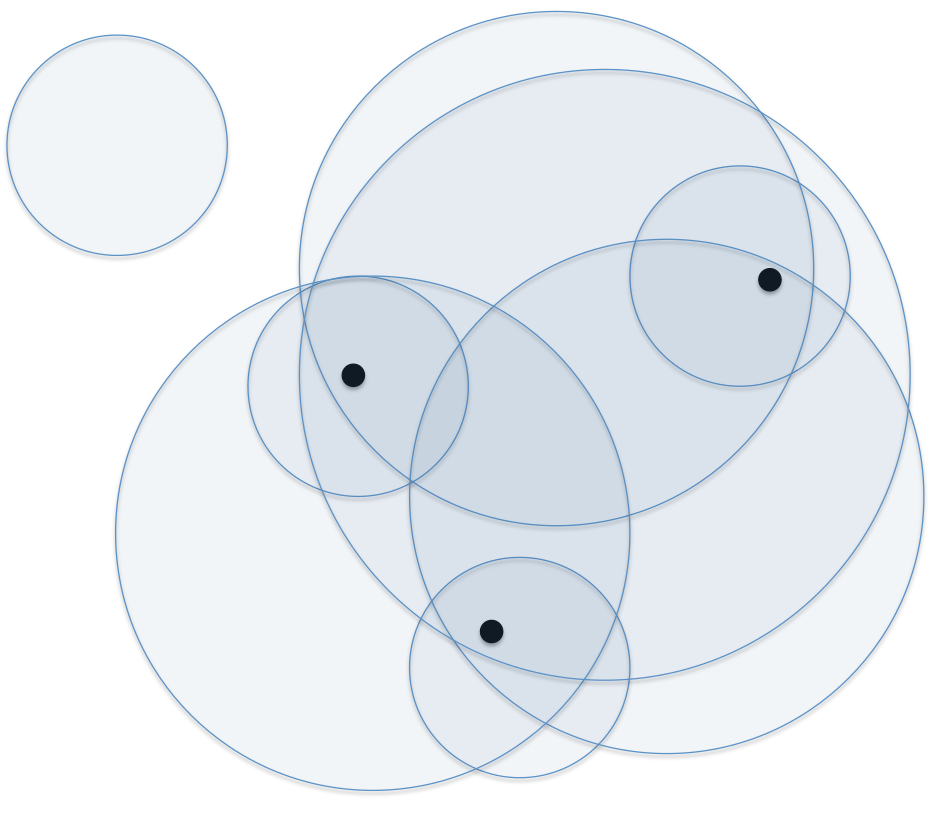
\includegraphics[width=5cm]{circles.png}
\end{figure}

%figure here

If we take n = 4, things start to get complicated. WE consider two cases:

\begin{itemize}
    \item If one of the 4 points, say $x_1$, lies within the convex hull of the other 3 points, then the labelling (0, 1, 1, 1) cannot be achieved.
    \item Otherwise, label the points in clockwise order $x_1, x_2, x_3, x_4$. Note that if there was a circle $c_1$ that achieves the label sequence 1, 0, 1, 0 and another circle $c_2$ that achieves the label sequence 0, 1, 0, 1 then their symmetric difference $c_1 \setminus c_2$ should consist of (at least) 4 disjoint regions. However, this is impossible for circles.
\end{itemize}

\textbf{Exercise 8.} Given some domain set, $\chi$ and a number $k \leq |\chi|$, compute the VC-dimension of the following hypothesis classes:

\begin{itemize}
    \item[a)] $H_{=k}^{\chi} = \{h \in \{0,1\}^k \ | \ |\{x|h(x) = 1\}| = k\}$, that is, the set of all functions that assign the value 1 to at most k elements of $\chi$.
    \item[b)] $H_{\leq k}^{\chi} = \{h \in \{0,1\}^k \ | \ |\{x|h(x) = 1\}| \leq k \text{ or } |\{x|h(x) = 0\}| \leq k \}$
\end{itemize}

\textbf{Solution.}

We will refer to the hypothesis classes as simply H in both subsections.

\begin{itemize}
    \item[a)] We claim that VCdim(H) = min\{k, $|\chi|$ - k\}.
    
    First, we show that VCdim(H) $\leq k$. Let $C \subset \chi$ be a set of size K + 1. Then, there doesn`t exist $h \in H$ that satisfies $h(x) = 1$ for all $x \in C$. Analogously, if $C \subset \chi$ is a set of size $|\chi| - k + 1$, there is no $h \in H$ which satisfies h(x) = 0 for all $x \in C$. Hence, VCdim(H) $\leq$ min\{k, $|\chi| - k$\}.
    
    It`s left to show that VCdim(H) $\geq$ min\{k, $|\chi| - k$\}. Let C = $\{x_1, ...,x_m\} \subset \chi$ be a set with size m $\geq$ min\{k, $|\chi| - k$\}. Let $\{x_1, ...,x_m\} \subset \{0,1\}^m$ be a vector of labels. Denote $\sum_{i=1}^{m} y_i = s$. Pick an arbitrarily subset $E \in \chi \setminus C$ of k - s elements and let $h \in H$ be a hypothesis which satisfies $h(x_i) = y_i, \forall x_i \in C$ and $h(x) = \textbf{1}_{[E]}, \forall x \in \chi \setminus C$. We conclude that C is shattered by H. It follows that VCdim(H) $\geq$ min\{k, $|\chi| - k$\}.
    
    \item[b)] We claim that VCdim(H) = k.
    
    First, we show that VCdim(H) $\leq k$. Let $C \subset \chi$ be a set of size k + 1. Then, $\nexists \ h \in H$ that satisfies h(x) = 1$, \forall x \in C$.
    
    It`s left to show that Vcdim(H) $geq$ k. Let C = $\{x_1, ...,x_m\} \subset \chi$ be a set of size $m \leq k$. Let $\{x_1, ...,x_m\} \subset \{0,1\}^m$ be a vector of labels. This labeling is obtained by some $h \in H$ which satisfies $h(x_i) = y_i, \forall x_i \in C$ and $h(x) = 0, \forall x \in \chi \setminus C$. We conclude that C is shattered by H. It follows that VCdim(H) $\geq k$. 
\end{itemize}

\vspace{3mm}

\textbf{Exercise 9.} Consider the class $\mathcal{H}^{d}_{mcon}$ of monotone Boolean conjunctions over $\{0,1\}^{d}$. Monotonicity here means that the conjunctions do not contain negations. As in $\mathcal{H}^{d}_{mcon}$, the empty conjunction is interpreted as the all-positive hypothesis. We augment $\mathcal{H}^{d}_{mcon}$ with the all-negative hypothesis $h^{-}$. Show that VCdim($\mathcal{H}^{d}_{mcon}$) = \textit{d}.

\textbf{Solution.}

$\hmc$ is the class of monotone Boolean conjunctions over $\szod$.
\begin{align*}
  \hmc =& \left\{
    h \col \szod \ra \szo,\, h_{(x_1, x_2, \dots, x_d)} =
     \bigwedge_{i=1}^d l(x_i)
  \right\}
     \cup
     \{ \usub{\downarrow \\ h^-(x_1, \dots, x_d) = 0\\ \text{ always}}{h^-} \} \\
     &
       \usub{\qquad\quad\;\downarrow\quad\downarrow\\
             \qquad\quad\text{positive}\quad{\text{missing}}\\
             \qquad\quad\text{literal}\;\;\quad\text{literal}}{l(x_i)\in \{x_i, 1\}}
\end{align*}

So $|\hmc| = 2^d + 1$.

Examples:
\begin{align*}
  d = 2 & \qquad
    \gH_{\text{mcon}}^2 =
      \{\usub{\downarrow\\h^-}{0}, \usub{\downarrow\\h_\text{empty}}{1}, x_1, x_2, x_1 \land x_2\} \\
  d = 3 & \qquad
    \gH_{\text{mcon}}^3 =
      \{0, 1, x_1, x_2, x_3, x_1 \land x_2, x_1 \land x_3, x_2 \land x_3, x_1 \land x_2 \land x_3\}
\end{align*}

We need to show that $\vcd{\hmc} = d$.

We know that $|\hmc| = 2^{d}+1$, so $\vcd{\hmc} \leq \floor{\log_2(|\hmc|)}$, which in turn means
\[\vcd{\hmc} \leq \floor{\log_2(2^{d}+1)} = d\]

We only need to find a set $C \subseteq \szod$ with $d$ points that is shattered by $\hmc$.

Usually, taking $C = \{e_1, e_2, \dots, e_d\}, e_i = (0, \dots, 0, 1, 0, \dots, 0)$ works, but
not for this $\gH = \hmc$. You cannot have a conjunction that will have
$h(e_1) = h(e_2) = 1$ and $h(e_3) = \dots = h(e_d) = 0$.

Instead, we choose $C = \{(0, 1, 1, \dots, 1), (1, 0, 1, 1, \dots, 1), \dots,
(1, 1, \dots, \uset{i}{0}, 1, 1)\}$ set of vectors of the form
${c_i = (1, 1, \dots, 1) - e_i, i = \overline{1, d}}$.

We want to show that, for each possible labeling $(y_1, y_2, \dots, y_d)$ of the points
$c_i = (1, 1, \dots, 1) - e_i$, there exists a function $h \in \hmc$ such that
$h(c_i) = y_i, \forall i = \overline{1, d}$.

Consider $(y_1, y_2, \dots, y_d)$ a labeling and take $\gJ = \{j \mid y_j = 1\}$.

If $\gJ = \emptyset$, then $h^-$ realizes the labeling $(0, 0, \dots, 0)$.

If $\gJ = \{1, 2, \dots, d\}$, then $h_\text{empty} = 1$ (all literals are missing) realizes the
labeling $(1, 1, \dots, 1)$.

If $1 \leq |\gJ| \leq d-1$, then consider
$h_{\gJ}(x_1, x_2, \dots, x_d) = \bigwedge\limits_{j \notin \gJ} x_j$.

For example, if $d = 4$ and $\gJ = \{2, 3\}$, $h_{\gJ}(x_1, x_2, x_3, x_4) = x_1 \wedge x_4$:
\begin{align*}
  h_{\gJ}(c_1) &= h_{\gJ}(0, 1, 1, 1) = 0 & \\
  h_{\gJ}(c_2) &= h_{\gJ}(1, 0, 1, 1) = 1 & \\
  h_{\gJ}(c_3) &= h_{\gJ}(1, 1, 0, 1) = 1 & \\
  h_{\gJ}(c_4) &= h_{\gJ}(1, 1, 1, 0) = 0 &
\end{align*}

We have that $h_{\gJ}(c_i) = 1$ if $i \in \gJ$ and $h_{\gJ}(c_i) = 0$ if $i \notin \gJ$.

For all indices $i \in \gJ$, $c_i$ will have value 0 on the position $i$ and 1 in rest, but
variable $x_i$ is not considered in the conjunction. So $h_{\gJ}(c_i) = 1$.

For all indices $i \notin \gJ$, $c_i$ will have value 0 on the position $i$ and, because the
conjunction contains the literal $x_i$, then we have that $h_{\gJ}(c_i) = 0$.

\vspace{3mm}

\textbf{Exercise 10.} Let $\mathcal{X}$ be the Boolean hypercube $\{0,1\}^n$. For a set $I \subseteq \{1, 2,\dots,n\}$ we define a \textit{parity function $h_I$} as follows. On a binary vector $x = (x_1, x_2, \dots, x_n) \in \{0,1\}^n$,

$$h_I(x) = \left( \sum_{i\in I} x_i \text{ mod 2} \right)$$

(That is, $h_I$ computes parity bits in $I$.) What is the VC-dimension of the class of all such parity functions, $\mathcal{H}_{n-parity} = \{h_I \ | \ I \in \{1, 2, \dots, n\}\}$?

\textbf{Solution.}

$\gX = \szon$

\[\hnp = \left\{h_I \mid  I \subseteq \sft{1, 2}{n},\; h_I(x_1, x_2, \dots, x_n) = 
\left(\sum_{i \in I} x_i\right) \mkern-10mu \mod 2\right\}\]

What is $\vcd{\hnp}$?

For each subset $I \subseteq \sft{1, 2}{n}$ we have a $h_I$, so $|\hnp| = 2^n$.

We know that $\vcd{\hnp} \leq \floor{\log_2 2^n} = n$.

So $\vcd{\hnp} \leq n$.

Can we find a set $C$ with $n$ points that is shattered by $\hnp$?

Let`s try the ``usual'' set of unit vectors $C = \{e_1, e_2, \dots, e_n\}, e_i = (0, \dots, 0, \uset{i}{1}, 0, \dots, 0)$.

We want to show that, for each possible labeling $(y_1, y_2, \dots, y_n)$ of $(e_1, e_2, \dots, e_n)$, you can find a corresponding
$h$ such that $h(e_i) = y_i, \forall i = \overline{1, n}$.

Consider $(y_1, y_2, \dots, y_n)$ such a labeling and take $I = \{i \mid y_i = 1\}$.

Then we have
\[
h_I(e_i) = \left(\sum_{i \in I} x_i\right) \mkern-10mu \mod 2 =
\begin{cases}
  1, & \text{if } i \in I \\
  0, & \text{otherwise}
\end{cases}
\]
So $\vcd{\hnp} = n$.

\vspace{3mm}

\textbf{Exercise 11.} Given some finite domain ser, $\mathcal{X}$, and a number $k \leq |\mathcal{X}|$, figure out the VC-dimension of each of the following classes (and prove your claims):

\begin{enumerate}
    \item $\mathcal{H}^{\mathcal{X}_{=k}}=\{h\in \{0,1\}^{\mathcal(X)} \ | \ |\{x \ | \ h(x)=1\} = k|\}$, that is, the set of all functions that assign the value of 1 to exactly \textit{k} elements of $\mathcal{X}$.
    \item $\mathcal{H}^{\mathcal{X}_{=k}}=\{h\in \{0,1\}^{\mathcal(X)} \ | \ |\{x \ | \ h(x)=1\} \leq k| \text{ or } |\{x \ | \ h(x)=0\} \leq k|\}$
\end{enumerate}

\textbf{Solution.}

$\gX$ is finite domain, $|\gX| < \infty$, $k \leq |\gX|$
\begin{flalign*}
\textbf{3.1. }\hkx{k} &=
  \left\{h \in \szo^{\gX} \;\vline\; |\{x \col h(x) = 1\}| = k\right\}& \\
&= \text{set of all functions that assign the value 1 to exactly } k \text{ elements of } \gX&
\end{flalign*}
$\vcd{\hkx{k}} = ?$

\begin{align*}
 &\text{If } k = 0 \Rightarrow \hkx{0} = \{h^-\}, \text{ all points get the value } 0 \\
 &\text{If } k = 1 \Rightarrow \hkx{1} \text{ has } |\gX| 
\text{ functions} = n \text{ functions} \\
& \qquad\gX = \{x_1, x_2, \dots, x_n\}, n = |\gX| \\
&\qquad h_i \col \{x_1, \dots, x_n\} \ra \szo \quad
h_i(x_j) = \begin{cases}
  1, & i = j \\
  0, & i \neq j
\end{cases} \\
 &\text{If } k = 2 \Rightarrow \hkx{2} \text{ has } C_n^2 \text{ elements} \\
 &\vdots \\
 &\text{If } k = n-1 \Rightarrow \hkx{n-1} \text { has } n \text{ elements} \\
 &\text{If } k = n \Rightarrow \hkx{n} \text{ has } 1 \text{ element } h^+(x_i) = 1 \; \forall i = \overline{1, n}
\end{align*}

\begin{tabbing}
We first show that \=$\vcd{\hkx{k}} \leq \min(k, n-k)$. \\
\>\qquad\rotatebox{90}{$=$} \\
\>$\vcd{\gH}$
\end{tabbing}

Case 1) if $n \geq 2k$, in this case, $\min(k, n-k) = k, \; k \leq \dfrac{n}{2}$

$\gH$ will consist of functions $h$ that label exactly $k$ elements of $\gX$ with label 1. So any set $C$ with more than $k$ points cannot be shattered because the labeling with all 1`s $(1, 1, 1, \dots, 1)$ cannot be realized by any $h \in \gH$.

Case 2) if $n < 2k$, in this case $\min(k, n-k) = n-k$, $k > \dfrac{n}{2}$

$\gH$ will consist of functions $h$ that labels $k$ elements of $\gX$ with label 1, and $n-k$ points of $\gX$ with label 0. So any set with more than $n-k+1$ points cannot be shattered by $\gH$ as the labeling with all 0`s $(0, 0, \dots, 0)$ cannot be realized by any $h \in \gH$.

So we have that $\vcd{\gH} \leq \min(k, n-k)$.

We will prove that $\vcd{\gH} = \min(k, n-k)$.

Consider $k'\ = \min(k, n-k)$.

We need to show that there exists a set of points ${A = \{x_{i1}, x_{i2}, \dots, x_{ik'}\} \subseteq \gX}$ that is shattered by $\gH$. This means that, for each subset $B \subseteq A$, we can find $h_B \in \gH$ such that
\[h_B(x)=
\begin{cases}
  1, & x \in B \\
  0, & x \in A \setminus B
\end{cases}
\]
We choose a set of $k - |B|$ points $B' = \{b_1, b_2, \dots, b_{k-|B|}\} \subseteq \gX \setminus A$.

\begin{flalign*}
\text{We can make the choice since }k - |B| &\leq |\gX \setminus A| &\\
k - |B| &\leq n-k' &\\
k' - |B| &\leq n-k &\\
k' - |B| &\leq k' \leq n-k \text{ (this is true)} &
\end{flalign*}
\begin{flalign*}
\text{So } B &\subseteq A \text{ has } |B| \text{ elements} &\\
B' &\subseteq \gX \setminus A \text{ has } k - |B| \text{ elements} &
\end{flalign*}
So $|B \cup B'| = |B| + |B'|$ (as $B \cap B' = \emptyset$) $ = k$

So, if we consider the characteristic function of the set $B \cup B'$, we have
\[
\sone_{B \cup B'}(x) =
  \begin{cases}
    1, & x \in B \cup B' \\
    0, & \text{otherwise}
  \end{cases}
\]
What is more important, $\sone_{B \cup B'}$ takes value 1 for exactly $k$ points, so it is a member of $\gH$.

So, in this case, we take $h_B = \sone_{B \cup B'}$.

$h_B$ will have the desired property that
$
h_B(x) =
  \begin{cases}
    1, & x \in B \\
    0, & x \in A \setminus B
  \end{cases}
$

So any set $A$ of $k' = min(k, n-k)$ points (?) can be shattered by $\gH$.

So $\vcd{\gH} = k' = \min(k, n-k)$.

\begin{flalign*}
\textbf{3.2. }\ham{k} &=
  \left\{h \in \szo^{\gX} \col |\{x \col h(x) = 1\}| \leq k \text{ or }|\{x \col h(x) = 0\}| \leq k\right\}&
\end{flalign*}

\begin{flalign*}
&\text{If } k = 0 \qquad \ham{0} = \{h^-, h^+\} \qquad
  \text{where }|\{x \col h^-(x) = 1\}| \leq 0 \text{ and } |\{x \col h^+(x) = 0\}| \leq 0& \\
&\text{If } k = 1 \qquad \ham{1} = \{h^-, h^+\} \cup \{\text{functions } h \text{ which label just one point with }\uset{\rotatebox[origin=c]{180}{$\Lsh$}\gH_{=1}^{\gX}}{\text{label 1}\}} &\\
&\hspace{14.9em}\cup \{\text{functions $h$ which label just one point with label 0}\} &
\end{flalign*}

\underline{Case 1}\qquad If $n = |\gX| \leq 2k-1$, then we have that
$\ham{k} = \szo^{\gX} = \{h \col ?? \gX \ra \szo\}$

This is true because any function $h \col \gX \ra \szo$ will have either at $\usub{\Downarrow\\h\in \ham{k}}{\text{most }k\text{ points}}$ labeled with 0 or at $\usub{\Downarrow\\h\in \ham{k}}{\text{most }k\text{ points}}$ labeled with 1.

Example (see Table \ref{tab:ex}): Take $n = 7, \; k = 4 \qquad \gX = \{x_1, x_2, x_3, x_4, x_5, x_6, x_7\}$
\begin{table}[h]
\centering
\begin{tabular}{lc|c|c|c|c|c|c|c}
&$x$    & $x_1$ & $x_2$ & $x_3$ & $x_4$ & $x_5$ & $x_6$ & $x_7$ \\
\cline{2-9}
at most \stackanchor{4 1`s}{4 0`s} $\leftarrow$ \quad &$h(x)$ &   1   &   1   &   0   &   0   &   1   &   0   &   1   \\
\cline{2-9}
at most 4 1`s $\leftarrow$ \quad &$h(x)$ &   0   &   0   &   1   &   0   &   0   &   0   &   0   \\
\cline{2-9}
at most 4 1`s $\leftarrow$ \quad &$h(x)$ &   0   &   1   &   0   &   0   &   1   &   0   &   0   \\
\cline{2-9}
\end{tabular}
\caption{}
\label{tab:ex}
\end{table}

In this case, $\vcd{\ham{k}} = \vcd{\szo}^{\gX} = n = |\gX|$.

\vspace{0.2cm}
\underline{Case 2}\qquad If $n = |\gX| \geq 2k+2$

We first show that $\vcd{\usub{\shortparallel\\\gH}{\ham{k}}} = \vcd{\gH} \geq 2k+1$

Consider any set $A$ of $2k+1$ points in $\gX$: $A = \{a_1, a_2, \dots, a_{2k+1}\}$.

We will show that $A$ is shattered by $\gH$. It is enough to show that, for each possible labeling $(y_1, y_2, \dots, y_{2k+1})$ of the points $(a_1, a_2, \dots, a_{2k+1})$, we can find an $h \in \gH$ such that $h(y_i) = a_i$.

Take $\gJ = \{j \mid y_j = 1\}$, and take $B_{\gJ} = \{a_j \in A \mid \uset{j \in \gJ}{y_j = 1}\}$

\begin{flalign*}
\text{If }|\gJ| \leq k \qquad &\text{we know that } \sone_{B_{\gJ}} \in \ham{k}\text{, so we take } \\&\qquad h = \sone_{B_{\gJ}} \quad
h(a_j) = \begin{cases}
  1, & y_j = 1 \\
  0, & \text{otherwise}
\end{cases} \\
\text{If }|\gJ| > k \qquad &\text{ take } C_{\gJ} = \{a_j \in A \mid \uset{j \notin \gJ}{y_j = 0}\} \text{ has at most }k \text{ elements, so we take in this case }\\&\qquad h = \sone_{A \setminus C_{\gJ}} \quad
h(a_j) = \begin{cases}
  1, & y_j = 1 \\
  0, & y_j = 0
\end{cases}
\end{flalign*}

So, we have that $\vcd{\gH} \geq 2k+1$.

We show now that $\vcd{\gH} < 2k+2$.

Consider any set $A$ of $2k+2$ points \quad $A = \{a_1, a_2, \dots, a_{2k+2}\}$.

There is no $h \in \gH$ that will label the first $k+1$ points with 1 and the rest $k+1$ points with 0.

So, in conclusion, $\vcd{\ham{k}} = \min(|\gX|, 2k+1)$.

\vspace{3mm}

\textbf{Exercise 12.} Let $\Sigma$ be a finite alphabet and let $\mathcal{X}=\Sigma^m$ be the sample space of all strings of length $m$ over $\Sigma$. Let $\mathcal{H}$ be a hypothesis space over $\mathcal{X}$, where $\mathcal{H}=\{h_{w}:\Sigma^m\to\{0,1\}, w \in \Sigma^*, 0 < |w| \leq m \text{ s.t. } h_w(x)=1 \text{ if } w \text{ is a substring of } x\}$. Give any upper bound for the VC-dimension of $\mathcal{H}$ in terms of $|\Sigma|$ and $m$.

\textbf{Solution.}

Solution 1:
\begin{proof}[Affirmation]\renewcommand{\qedsymbol}{}
$VCDim(\mathcal{H}) < |\Sigma|^m$
\end{proof}

\begin{proof}

Let $m\in\mathbb{N}^*$ and $\Sigma$, $\mathcal{X}$ and $\mathcal{H}$ defined as above. Assume that $VCDim(\mathcal{H})\geq|\Sigma|^m$, then $\mathcal{H}$ should shatter a set of $|\Sigma|^m$ distinct words from $\mathcal{X}$ and the only such set is $\mathcal{X}$ itself. Take the $(\underbrace{0, 0, ..., 0}_{|\Sigma|^m})$ labeling, then there should be a $h_w\in\mathcal{H}$ such that $w$ does not exist as a substring for every word in $\mathcal{X}$. 

If $m=1$ and $|\Sigma|=1$, assume that $\mathcal{X}=\{a\}$, then $\mathcal{H}=\{h_a\}$ since we can`t have $|w|=0$, so the $(0)$ label is not possible.

If $m>1$ and $|\Sigma|=1$, assume that $\mathcal{X}=\{\underbrace{aa...a}_m\}$, then $\mathcal{H}=\{h_{\underbrace{aa...a}_{j}}\ | 1 \leq j \leq m\}$, so the $(0)$ label is not possible.

In general, if $m\geq1$ and $|\Sigma|\geq1$ pick any $h_w \in \mathcal{H}$ and let $n$ be the length of $w$. Since $\mathcal{X}$ contains every possible word of length $m$, it will also contain the word $w+\underbrace{v...v}_{m-n}$, where $+$ is the concatenation operator and $v$ is any letter in $\Sigma$, so there will always be at least one element labeled with $1$, thus the labeling $(\underbrace{0, 0, ..., 0}_{|\Sigma|^m})$ is not possible, so $\mathcal{H}$ can`t shatter $\mathcal{X}$ and we get a contradiction with the assumption that $VCDim(\mathcal{H})\geq |\Sigma|^m$.
\end{proof}

Solution 2:
\begin{proof}[Affirmation]\renewcommand{\qedsymbol}{}
$VCDim(\mathcal{H}) \leq log_2(|\mathcal{H}|) = log_2(|\Sigma|^1+|\Sigma|^2+...+|\Sigma|^m)$
\end{proof}

\begin{proof}
The class $\mathcal{H}$ has cardinality $|\mathcal{H}| = |\Sigma|^1+|\Sigma|^2+...+|\Sigma|^m$ - it contains all the hypothesis $h_w$ where $w$ is a word of maximum length $m$ with elements from $\Sigma$, so $\mathcal{H}$ is a finite class. By observation $6.3.4$ from \cite{SS}, we have that $VCDim(\mathcal{H}) \leq log_2(|\mathcal{H}|) = log_2(|\Sigma|^1+|\Sigma|^2+...+|\Sigma|^m)$.
\end{proof}

\textbf{Exercise 13. (Duality of VC dimension)} Let $\chi$ be an instance space and $H \subseteq \{0,1\}^X$ a hypothesis space with finite VC dimension. For each $x \in \chi$, we consider the function $z_x : H \rightarrow \{0,1\}$ such that $z_x(h) = h(x)$ for each $h \in H$. Let $Z = \{z_x : H \rightarrow \{0,1\} \ | \ x \in \chi\}$. Prove that $VCdim(Z) < 2^{VCdim(H) + 1}$.

\textbf{Solution.}

We will prove that $VCdim(Z) < 2^{VCdim(H) + 1}$ by contradiction.

We start by giving the following equivalent \textbf{definition}\cite{signvcvcdim}:

\textit{The VC dimension of a binary matrix $S$, denoted $VC(S)$, is defined as follows. A subset $C$ of columns of $S$ is called shattered if each of the $2^{|C|}$ different patterns of ones and zeroes appears in some row in the restriction of $B$ to the columns in $C$. The VC dimension of $B$ is the maximal size of a shattered subset of columns.} 

Let $VCdim(H) = d$. \hspace{7.7cm} (1)

Suppose that $VCdim(Z) \geq 2^{d+1}$. 

$\exists \mathcal{Y} \subset H, |\mathcal{Y}|=2^{d+1}$ a subset of functions and $Y \subset X, |Y| = 2^{2^{d+1}}$ a subset of points, s.t. the vectors $(z_1(x) \dots z_{|\mathcal{Y}|}(x))$ range over all possible $2^{2^{d+1}}$ binary combinations as $x$ ranges over the points in Y. 

We construct the matrix $A$ by queueing all $(z_1(x) \dots z_{|\mathcal{Y}|}(x))$ vectors one after another as its columns. The  first row will be comprised of $z_1$ functions, the second row will hold $z_2$ functions and so on until row $2^{d+1}$ which will hold the $z_{|\mathcal{Y}|}$ functions. The resulting matrix will be of shape $2^{d+1} \times 2^{2^{d+1}}$, with rows indexed after elements of $\mathcal{Y}$ and columns indexed after elements of $Y$. 

$A$ is a row-wise representation of $\mathcal{Y}$ and a column-wise representation of $Y$.

We denote with $B$ the $2^{d+1} \times (d+1)$ matrix whose rows are binary digits of the numbers raging from 0 to $2^{d+1} - 1$. In other words, we number the rows using binary digits of length $d+1$. In particular, we have that for each $i$ there is a column that contains the $i^{th}$ bit of the row index.

For example, for $d = 2$, we have:

\[B = 
\begin{pmatrix}
0 & 0 & 0 \\
0 & 0 & 1 \\
0 & 1 & 0 \\
0 & 1 & 1 \\
1 & 0 & 0 \\
1 & 0 & 1 \\
1 & 1 & 0 \\
1 & 1 & 1 
\end{pmatrix} \text{, where rows represent numbers from 0 to 7.}
\]

We know from the re-interpretation of VC dimension for binary matrices that the VC dimension of $A$ is the maximal size of a set $S$ of columns which are shattered, that is, all possible rows appear when we restrict $A$ to the columns in $S$.

Since the columns of $A$ contain all possible binary vectors of length $2^{d+1}$, then $B$ must be a submatrix of $B$. This means that $VCdim(A) = d + 1$, which is the number of columns of $B$.

Since the rows of $A$ are indexed after elements of $\mathcal{Y}$, $A$ is a row-wise binary representation of $H$. Thus, there exists a set of points of size $d+1$ which is shattered by H and therefore $VCdim(H) \geq d+1$. \hspace{4.8cm} (2)

\vspace{1mm}

$(1) + (2) \Rightarrow \bot$. So $VCdim(Z) < 2^{d+1}$, with $d = VCdim(H)$.

\newpage

\section{Shattering Coefficient}

\textbf{Exercise 1.} Consider the following hypothesis class:

$$H = \{h_{\theta_{1}} : \mathbb{R} \rightarrow \{0,1\} \ | \ h_{\theta_{1}} = \textbf{1}_{[\theta_1, \infty)}, \theta_1 \in \mathbb{R}\} \ \cup \ \{h_{\theta_{2}} : \mathbb{R} \rightarrow \{0,1\} \ | \ h_{\theta_{2}} = \textbf{1}_{(-\infty, \theta_2)}, \theta_2 \in \mathbb{R}\}$$

\begin{itemize}
    \item[a)] Compute the shattering coefficient $\tau_H(m)$ of the growth function for m$>$0.
    \item[b)] Compare your result with the general upper bound for growth functions.
    \item[c)] Does there exist a hypothesis class H for which $\tau_H(m)$ is equal to the general upper bound? If you answer is yes, provide an example. If your answer is no, provide a justification.
\end{itemize}

\textbf{Solution.}

a) Consider the following hypothesis classes:

$$H_{thresholds}^{1} = \{h_{\theta_{1}} : \mathbb{R} \rightarrow \{0,1\} \ | \ h_{\theta_{1}} = \textbf{1}_{[\theta_1, \infty)}, \theta_1 \in \mathbb{R}\}$$

and

$$H_{thresholds}^{2} = \{h_{\theta_{2}} : \mathbb{R} \rightarrow \{0,1\} \ | \ h_{\theta_{2}} = \textbf{1}_{(-\infty, \theta_2)}, \theta_2 \in \mathbb{R}\}$$

Obviously for each of these classes we have that $\tau_H(m) = m + 1$. Let`s look at all the possible labelings with $H_{thresholds}^{2}$. Let $L^2$ be the set of all possible labelings with $H_{thresholds}^{2}$. We have that:

$$L^2 = \{(0, 0, 0, \dots , 0), (1, 0, 0, \dots ,0), (1, 1, 0, \dots, 0), \dots, (1, 1, 1, \dots, 1)\}$$

It`s easy to observe that $|L^2| = m + 1$. There are m labelings that contain at least one 1 label, plus $(0, 0, \dots, 0)$. If we swap the order of the 1s, we get all labelings for $H_{thresholds}^{1}$. Let $L^1$ be the set of all possible labeling for $H_{thresholds}^{1}$. We have:

$$L^1 = \{(0, 0, 0, \dots , 0), (0, 0, 0, \dots , 1), (0, \dots, 0, 1, 1), \dots, (1, \dots, 1, 1, 1)\}$$

Now, since $H = H_{thresholds}^{1} \cup H_{thresholds}^{2}$, we have $L = L^1 \cup L^2$ the set of all possible labelings of m points with H. We have that:

\[
\begin{aligned}
    L = \{& (0, 0, 0, \dots , 0), (1, 0, 0, \dots ,0), (1, 1, 0, \dots, 0), \dots, (1, 1, 1, \dots, 1), \\
    & (0, 0, 0, \dots , 0), (0, 0, 0, \dots , 1), (0, \dots, 0, 1, 1), \dots, (1, \dots, 1, 1, 1)\}
\end{aligned}
\]

The only common elements are $(0, 0, \dots, 0)$ and $(1, 1, \dots, 1)$, so have that:

\[
\begin{aligned}
    \tau_{H}(m) & = \tau_{H_{thresholds}^{1}}(m) + \tau_{H_{thresholds}^{2}}(m) \\
    & = m + 1 + m + 1 - 2 \\
    & = 2m.
\end{aligned}
\]

b) By the Sauer-Shelah-Perles lemma, we have that $\tau_H(m) \leq \sum_{i=0}^{d} {m \choose i}$, where $d = VCdim(H)$.

We know from the last assignment that VCdim(H) = 2, so:
\[
\begin{aligned}
    \tau_H(m) & \leq \sum_{i=0}^{2} {m \choose i}\\
    & \leq {m \choose 0} + {m \choose 1} + {m \choose 2}\\
    & \leq \frac{m!}{0!(m-0)!} + \frac{m!}{1!(m-1)!} + \frac{m!}{2!(m-2)!} \\
    & \leq 1 + m + \frac{m(m-1)}{2}.
\end{aligned}
\]

This shows that our result, $\tau_H(m) = m + 1$, is considerably smaller than the general upper bound for growth functions.

c) Recall that $H_{thresholds}^{1}$ and $H_{thresholds}^{2}$ have shatter coefficient of $\tau_H(m) = m + 1$. Let H be one of the classes mentioned a priori. Now we set $d = VCdim(H) = 1$. By Sauer`s lema we have that:

$$\tau_H(m) \leq {m \choose 0} + {m \choose 1} = \frac{m!}{0!(m-0)!} + \frac{m!}{1!(m-1)!} = 1 + m.$$ 

So the upper bound of the shatter coefficient of H is equal to $\tau_H(m)$.

\vspace{3mm}

\textbf{Exercise 2.} Consider the concept class H formed by closed intervals [a,b] with $a,b \in \mathbb{R}$:
\vspace{-1mm}
$$H = \{h_{a,b} : \mathbb{R} \rightarrow \{0, 1\} \ | \ h_{a,b} = \textbf{1}_{[a,b]}(x), a \leq b\}$$

Compute the shattering coefficient $\tau_H(m)$ of the growth function for $m \geq 0$.

\textbf{Solution.}

We start by denoting the concept class with H so that we can use the same notations as in \textit{Understanding Machine Learning} (Shai Ben-David, Shai Shalev-Shwartz) without causing any confusion: 
\vspace{-1mm}
$$H = \{h_{a,b} : \mathbb{R} \rightarrow \{0, 1\} \ | \ h_{a,b} = \textbf{1}_{[a,b]}(x), a \leq b\}$$

Let $C \subset \mathbb{R}, C = \{c_i \ | \ c_i \in \mathbb{R} \, c_j \neq c_k, \forall j,k, j \neq k\},|C| = m$.

We have two cases for $H \cap C$:

\begin{enumerate}
    \item $H \cap C = \{c_i, \dots , c_j\}$, with $1 \leq i \leq j \leq m$. 
    %\item $H \cap C \neq \varnothing$
    \item $H \cap C = \varnothing$. 
\end{enumerate}

We will start with the second case as it is simpler. The empty set denotes that there are no 1-labeled points, so $H \cap C$ creates the labeling $\underbrace{(0, 0, \dots , 0)}_\text{m elements}$.

Regarding the first case, there are ${m+1 \choose 2}$ possible labelings. The 1-labeled points need to be consecutive due to the nature of intervals, so we have:

\begin{itemize}
    \centering
    \item[] $\underbrace{\{(1, 0, 0, \dots , 0), (0, 1, 0, \dots, 0), (0, 0, 1, \dots, 0) \dots (0, 0, 0, \dots , 1)\}}_\text{\normalsize m labelings with 1 1-labeled point.}$
    
    \item[] 
    $\underbrace{\{(1, 1, 0, \dots  ,0, 0), (0, 1, 1, \dots, 0, 0) \dots (0, 0, 0, \dots , 1, 1)\}}_\text{\normalsize m - 1 labelings with 2 1-labeled points.}$
    
    \item[] 
    $\underbrace{\{(1, 1, 1, 0 \dots  0, 0, 0, 0), (0, 1, 1, 1, \dots, 0, 0, 0, 0) \dots (0, 0, 0, \dots ,0, 1, 1, 1)\}}_\text{\normalsize m - 2 labelings with 3 1-labeled points.}$

    \item[] \dots\dots\dots\dots\dots\dots\dots\dots\dots\dots\dots\dots\dots\dots\dots\dots\dots\dots\dots\dots
    
    \item[] 
    $\underbrace{\{(1, 1, 1, \dots  , 1, 0, 0), (0, 1, 1, \dots, 1, 1, 0) \dots (0, 0, 1, \dots , 1, 1, 1)\}}_\text{\normalsize 3 labelings with m-2 1-labeled points.}$
    
    \item[]
    $\underbrace{\{(1, 1, \dots  , 1, 0), (0, 1, \dots, 1, 1)\}}_\text{\normalsize 2 labelings with m-1 1-labeled points.}$
    
    \item[]
    $\underbrace{\{(1, 1, \dots  , 1, 1)\}}_\text{\normalsize 1 labeling with m 1-labeled points.}$
    
\end{itemize}

In total we have $m + (m-1) + $\dots$ + 1 \xlongequal{Gauss' formula} \frac{m\cdot(m+1)}{2} = {m+1 \choose 2}$. By adding the $(0, 0, \dots, 0)$ labeling from the $2^{nd}$ case, we get ${m+1 \choose 2} + 1$ labelings.

Thus, $\tau_H(m) = {m+1 \choose 2} + 1$.

\newpage

\section{Boosting}

\textbf{Exercise 1.} Consider the boosting algorithm described (page 4) in the article "\href{https://www.cs.cmu.edu/~efros/courses/LBMV07/Papers/viola-cvpr-01.pdf}{Rapid object detection using a boosted cascade of simple features}", P. Viola and M. Jones, CVPR 2001. Consider that the number of positives is equal with the number of negative examples (l = m).

\begin{itemize}
    \item[a.] Prove that the distribution $w_{t+1}$ obtained at round t + 1 based on the algorithm described in the article is the same with the distribution $D_{(t+1)}$ obtained based on the procedure described in the following figure:
    \begin{figure}[h]
        \centering
        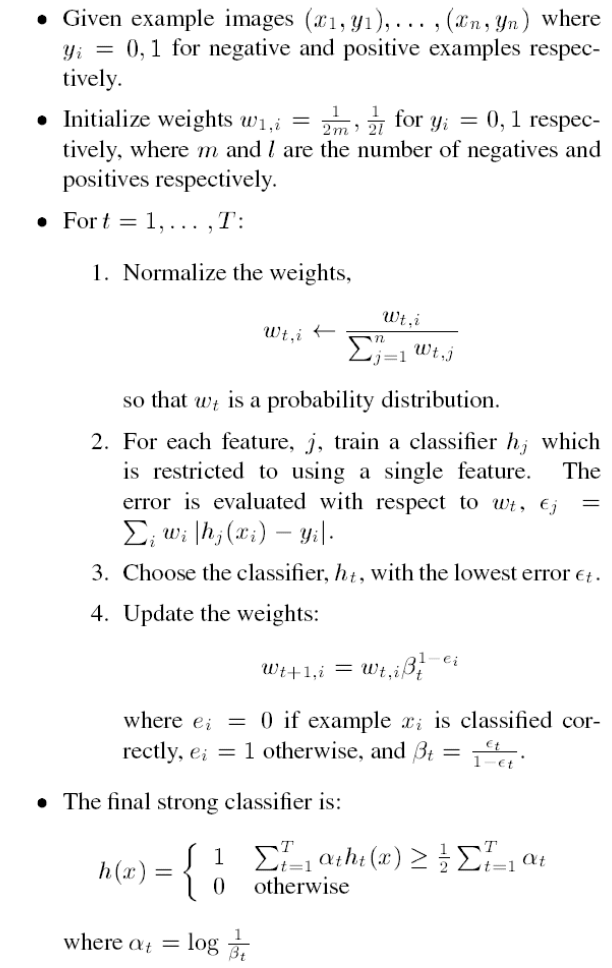
\includegraphics[width=7.5cm]{adaboost.png}
    \end{figure}
    \item[b.] Prove that the two final classifiers (the one described in the article and the one described in the previous figure) are equivalent.
    \item[c.] Assume that at each iteration t of AdaBoost, the weak learner returns a hypothesis $h_t$ for which the error $\epsilon_t$ satisfies $\epsilon_t \leq 1/2 – \gamma, \gamma > 0$. What is the probability that the classifier $h_t$ (selected as the best weak learner at iteration t) will be selected again at iteration t+1? Justify your answer.
\end{itemize}

\textbf{Solution.}

a) In the Viola-Jones version of AdaBoost, the distribution $w_{t+1, i}$ is of form:
$$w_{t+1, i} = \frac{w_{t, i}}{\sum_{j=1}^{n} w_{t, j}} \cdot \beta_t^{1 - |h_t(x_i) - y_i|} = \frac{w_{t, i}}{\sum_{j=1}^{n} w_{t, j} \cdot \beta_t^{|h_t(x_i) - y_i| - 1}}.$$

There are two possibilities for every element in the denominator sum:

\begin{enumerate}
    \item $h_t(x_i) \neq y_i$. The power of $\beta_t$ is 0, so the weight $w_{t,j}$ stays the same.
    \item $h_t(x_i) = y_i$. The weight $w_{t,j}$ becomes smaller by dividing it with $\beta_t$.
\end{enumerate}

Note that we used $|h_t(x_i) - y_i|$ to simulate $e_i$.

We will further prove that the final version of the $D_{t+1,i}$ distribution from the Freund-Schapire version of AdaBoost is equal to $w_{t+1, i}$. Before that, however, we need to make a couple of remarks:

\begin{itemize}
    \item $h_t(x_i)\cdot y_i$ has the same output for $y_i \in \{-1, +1\} \text{ and } h : \mathbb{R}^n \rightarrow \{-1,+1\}$, as $|h_t(x_i) - y_i|$ for $y_i \in \{0, 1\} \text{ and } h : \mathbb{R}^n \rightarrow \{0,1\}$.
    \item In both versions, the error $\epsilon_t$ is computed in the same way. Additionally, we will refer to $\frac{\epsilon_t}{1 - \epsilon_t}$ as $\beta_t$ for both AdaBoost versions, as it will simplify explanations.
\end{itemize}

Now we move on to computing $D_{t+1,i}$:
\[
\begin{aligned}
    D_{t+1, i} & = \frac{D_{t,i}}{Z_{t+1}} \cdot \beta_t^{-\frac{1}{2}h_t(x_i)y_i}\\
    & = \frac{D_{t,i}}{\sum_{j=1}^{N} D_{t,j} \cdot \beta_t^{-\frac{1}{2}h_t(x_j)y_j}} \cdot \beta_t^{-\frac{1}{2}h_t(x_i)y_i} \\
    & = \frac{D_{t,i}}{\sum_{j=1}^{N} D_{t,j} \cdot \beta_t^{\frac{1}{2}h_t(x_i)y_i-\frac{1}{2}h_t(x_j)y_j}}\\ 
    & = \frac{D_{t,i}}{\sum_{j=1}^{N} D_{t,j} \cdot \beta_t^{\frac{1}{2} (h_t(x_i)y_i - h_t(x_j)y_j)}}
    .
\end{aligned}
\]

\newpage

In the Freund-Schapire version we have two cases for each element of the denominator sum:
\vspace{-1mm}
\begin{enumerate}
    \item $h_t(x_i)y_i = h_t(x_j)y_j$. The power of $\beta_t$ is 0, meaning that the element $D_{t, j}$ stays the same.
    \item $h_t(x_i)y_i \neq h_t(x_j)y_j$. Then $\beta_t^{\frac{1}{2} (h_t(x_i)y_i - h_t(x_j)y_j)} = \beta_t^{\frac{1}{2} \cdot (-2)} = \beta_t^{-1}$. Thus the weight $D_{t,j}$ becomes smaller by dividing it with $\beta_t$.
\end{enumerate}

As one can see, case 1 and 2 for the Viola-Jones version map perfectly with their respective cases from the Freund-Schapire version of AdaBoost. Either the weight stays the same, as for case 1, or it is divided by $\beta_t$, as in case 2.

This concludes our proof that $w_{t+1,i}$ is the same as $D_{t+1,i}$.

\vspace{1mm}

b) For the Viola-Jones version of AdaBoost, we have:
\[
\begin{aligned}
    \sum_{t = 1}^{T} ln(\beta_t) h_t(x) \geq \frac{1}{2} \sum_{t=1}^{T} ln(\beta_t) & \Leftrightarrow \\
    \sum_{t = 1}^{T} ln(\beta_t) h_t(x) \geq  \sum_{t=1}^{T} \frac{1}{2} ln(\beta_t) & \Leftrightarrow \\
    \sum_{t = 1}^{T} ln(\beta_t) h_t(x) - \sum_{t=1}^{T} \frac{1}{2} ln(\beta_t) \geq 0 & \Leftrightarrow \\
    \sum_{t = 1}^{T} ln(\beta_t) h_t(x) - \frac{1}{2} ln(\beta_t) \geq 0 & \Leftrightarrow \\
    \sum_{t = 1}^{T} ln(\beta_t) \cdot (h_t(x) - \frac{1}{2}) \geq 0.
\end{aligned}
\]

We can rewrite the Viola-Jones strong classifier as follows:

$$h(x)=
\begin{cases}
1, \ \sum_{t = 1}^{T} ln(\beta_t) \cdot (h_t(x) - \frac{1}{2}) \geq 0\\
0, \text{ otherwise}
\end{cases}
$$

We also rewrite the Freund-Schapire strong classifier $h(x) = sign(\sum_{t=1}^{T} w_t h_t(x))$:

$$h(x)=
\begin{cases}
+1, \ \sum_{t=1}^{T} ln(\beta_t) \cdot \frac{1}{2} \cdot h_t(x) \geq 0\\
-1, \text{ otherwise}
\end{cases}
$$

Since $h_t(x) \in \{0, 1\}$ for the Viola-Jones version and $h_t(x) \in \{-1, +1\}$ for the Freund-Schapire version, this means that $h_t(x) - \frac{1}{2}$ in the Viola-Jones version is equivalent to $\frac{1}{2} \cdot h_t(x)$ in the Freund-Schapire version. The role of both is to determine the sign of $ln(\beta_t), \forall t = \overline{1, T}$ and divide it by 2.

Given that we know from \textbf{a)} that the distributions $w_{t,i}$ and $D_{t,i}$ are the same, this means that the values of the betas are the same. 

With this, we have proven that the two version of AdaBoost are equivalent.

c) \begin{proof}[Affirmation]\renewcommand{\qedsymbol}{}
$\mathbb{P}(h_t=h_{t+1})=0$.
\end{proof}
\begin{proof}
Assume that $\mathbb{P}(h_t=h_{t+1})>0$ and pick the $h_t$ and $h_{t+1}$ such that $h_t = h_{t+1}$, let $m$ be the size of the training set. 

We have that

\begin{equation}
\varepsilon_t = \sum\limits_{\substack{1\leq i \leq m\\ h_t(x_i)\neq y_i}} D_i^{(t)}    
\end{equation}

And, because we do normalization, we have that $D^{(t)}$ is a probability distribution, hence:

\begin{align}
    1 &= \sum_{i=1}^m D_i^{(t)}
      \\&= \sum\limits_{\substack{1\leq i \leq m\\h_t(x_i)\neq y_i}}D_i^{(t)} + \sum\limits_{\substack{1\leq i \leq m\\h_t(x_i) = y_i}}D_i^{(t)}
      \\&= \varepsilon_t + \sum\limits_{\substack{1\leq i \leq m\\h_t(x_i) = y_i}}D_i^{(t)}
\end{align}

Now, consider the error $\varepsilon_{t+1}$:

\begin{equation}
\varepsilon_{t+1} = \sum\limits_{\substack{1\leq i \leq m\\ h_{t+1}(x_i)\neq y_i}} D_i^{(t+1)} 
\stackrel{(17)}{=}
\frac{ \sum\limits_{\substack{1\leq i \leq m\\ h_{t+1}(x_i)\neq y_i}} 
 D_i^{(t)} }
{\sum\limits_{\substack{1\leq j \leq m\\ h_{t}(x_j) = y_j}}
D_j^{(t)}\frac{\varepsilon_t}{1-\varepsilon_t} +
\sum\limits_{\substack{1\leq j \leq m\\ h_{t}(x_j)\neq y_j}}
D_j^{(t)}
}
\end{equation}

But we assumed that $h_t = h_{t+1}$, hence:

\begin{align}
\varepsilon_{t+1} &= 
\frac{ \sum\limits_{\substack{1\leq i \leq m\\ h_{t}(x_i)\neq y_i}} 
 D_i^{(t)} }
{\sum\limits_{\substack{1\leq j \leq m\\ h_{t}(x_j) = y_j}}
D_j^{(t)}\frac{\varepsilon_t}{1-\varepsilon_t} +
\sum\limits_{\substack{1\leq j \leq m\\ h_{t}(x_j)\neq y_j}}
D_j^{(t)}
}
\\&\stackrel{(25)}{=}
\frac{ \varepsilon_t}
{\frac{\varepsilon_t}{1-\varepsilon_t}\sum\limits_{\substack{1\leq j \leq m\\ h_{t}(x_j) = y_j}}
D_j^{(t)} +
\varepsilon_t
}
\\&\stackrel{(28)}{=}
\frac{ \varepsilon_t}
{\frac{\varepsilon_t}{1-\varepsilon_t}(1-\varepsilon_t) +
\varepsilon_t
}
\\&=\frac{\varepsilon_t}{2\varepsilon_t}
\\&=\frac{1}{2}
\end{align}

But from the hypothesis, we have that $\forall t \in \mathbb{N}$, $\varepsilon_t \leq \frac{1}{2} - \gamma$, where $\gamma > 0$, so $\varepsilon_{t+1} < \frac{1}{2}$, which is a contradiction with (34), so our assumption that $\mathbb{P}(h_t = h_{t+1})>0$ is incorrect. It remains, therefore, that $\mathbb{P}(h_t=h_{t+1})=0$.

\end{proof}

\textbf{Exercise 2.} Let A be a 24 x 24 matrix representing an image. The integral image of A, denoted by I(A), is the matrix B such that $B_{i,j} = \sum_{i' \leq i, j' \leq j} A_{i,j}$ .

\begin{itemize}
    \item[a)] Show that I(A) can be calculated from A in linear time in size of A.
    \item[b)] Show how every Viola and Jones feature can be calculated from I(A) in a constant amount of time (that is, the runtime does not depend on the size of the rectangle defining the feature).
\end{itemize}

\textbf{Solution.}

a) We apply dynamic programming. Let $A \in \mathbb{R^{n x n}}$. First, observe that filling sequentially each item of the first column and the first row of I(A) can be done in a constant time. Next, given i, j $\geq$ 2, we note that $I(A)_{i,j} = I(A)_{i-1,j} + I(A)_{i,j-1} - I(A)_{i-1,j-1}$. Hence, filling the values of I(A), row by row, can be done in time linear in the size of I(A).

b) We show the calculation of type B. The calculation of the other types is done similarly. Given $i_1 < i_2 , j_1 < j_2$, consider the following rectangular regions:

\begin{itemize}
    \item[] $A_U = \{(i,j) \ | \ i_1 \leq i \leq \lfloor \frac{i_1 + i_2}{2} \rfloor \, j_1 \leq j \leq j_2\}$
    \item[] $A_D = \{(i,j) \ | \ \lceil \frac{i_1 + i_2}{2} \rceil \leq i \leq i_2, j_1 \leq j \leq j_2\}$
\end{itemize}

Let $b \in \{-1, 1\}$ and h be a hypothesis. That is, $h(A) = b \cdot (\sum_{(i,j) \in A_L} A_{i,j} - \sum_{(i,j) \in A_R} A_{i,j})$. Let $i_3 = \lfloor \frac{i_1 + i_2}{2} \rfloor$ and $i_4 = \lceil \frac{i_1 + i_2}{2} \rceil$. Then:

$$h(A) = B_{i_2, j_2} - B_{i_3, j_2} - B_{i_2, j_1 - 1} + B_{i_3, j_1 - 1} - (B_{i_3, j_2} - B_{i_1 - 1, j_2} - B_{i_3, j_1 - 1} + B_{i_1 - 1, j_1 - 1})$$

We conclude that h(A) can be calculated in constant time given B = I(A).

\vspace{3mm}

\textbf{Exercise 3.} Fix $\epsilon \in \left(0, \dfrac{1}{2}\right)$. Let the training sample be denoted by
$m$ points in the plane with $\dfrac{m}{4}$ negative points all at coordinate $(+1, +1)$,
another $\dfrac{m}{4}$ negative points all at coordinate $(-1, -1)$,
$\dfrac{m(1+\epsilon)}{4}$ positive points all at coordinate $(-1, +1)$,
$\dfrac{m(1-\epsilon)}{4}$ positive points all at coordinate $(+1, -1)$.

\begin{enumerate}[label=\alph*.]
  \item[a.] Describe the behavior of AdaBoost when run on this sample using boosting stumps
  for the first two rounds.
  \item[b.] What is the error of the optimal classifier chosen at round 1 in the second round?
\end{enumerate}

\textbf{Solution.} 

\begin{center}
{\Large AdaBoost}
\end{center}

• \, construct distribution $\bdt$ on $\som$:

\quad • \, $\bdoi = 1/m$

\quad • \, given $\bdt$ and $h_t$: $\dtti = \dfrac{\dti \times e^{-w_t h_t(x_i)y_i}}{Z_{t+1}}$

where $\zto$ normalization factor ($\bdtt$ is a distribution):
$\zto = \sum\limits_{i=1}^m \dti \times e^{-w_t h_t(x_i)y_i}$
\begin{align*}
&w_t \text{ is a weight: } w_t = \frac{1}{2}\ln\left(\frac{1}{\epsilon_t}-1\right)>0
  \text{ as the error } \epsilon_t < 0.5 \\
&\epsilon_t \text{ is the error of } h_t \text{ on } \bdt:
  \epsilon_t = \text{Pr}_{i \sim \dt}[h_t(x_i) \neq y_i] =
  \sum_{i=1}^m \dti \times \sone_{[h_t(x_i) \neq y_i]}
\end{align*}

If example $\rvx_i$ is correctly classified, then $h_t(\rvx_i) = \ry_i$, so at the next
iteration $t+1$ its importance (probability distribution) will be decreased to:
\[
\dtti = \frac{\dti \times e^{-w_t}}{\zto} =
  \dfrac{\dti \times e^{-\frac{1}{2}\ln\left(\frac{1}{\epsilon_t}-1\right)}}{\zto} =
  \dfrac{\dti \times \left(\frac{1}{\epsilon_t}-1\right)^{-\frac{1}{2}}}{\zto} =
  \dfrac{\dti \times \sqrt{\frac{\epsilon_t}{1-\epsilon_t}}}{\zto}
\]

If example $\rx_i$ is misclassified, then $h_t(\rx_i) \neq \ry_i$, so at the next
iteration $t+1$ its importance (probability distribution) will be increased to:
\[
\dtti = \frac{\dti \times e^{w_t}}{\zto} =
  \dfrac{\dti \times e^{\frac{1}{2}\ln\left(\frac{1}{\epsilon_t}-1\right)}}{\zto} =
  \dfrac{\dti \times \left(\frac{1}{\epsilon_t}-1\right)^{\frac{1}{2}}}{\zto} =
  \dfrac{\dti \times \sqrt{\frac{1-\epsilon_t}{\epsilon_t}}}{\zto}
\]

\begin{proof}[Solution]

%% otherwise the solution text comes down next to the minipage
\phantom{.}

\noindent
\begin{minipage}{0.5\textwidth}
\begin{tikzpicture}
    \draw[->] (-2,0) -- (2,0);
    \draw[->] (0,-2) -- (0,2);
    
    \draw (1,1) node[circle,draw,inner sep=0] {$-$} node[right=0.2,scale=0.9] {$\frac{m}{4}$ points} node[above=0.2] {(1,1)};
    \draw (1,-1) node[circle,draw,inner sep=0] {$+$} node[right=0.2,scale=0.9] {$\frac{m(1-\epsilon)}{4}$ points} node[below=0.2] {(1,-1)};
    \draw (-1,-1) node[circle,draw,inner sep=0] {$-$} node[left=0.2,scale=0.9] {$\frac{m}{4}$ points} node[below=0.2] {(-1,-1)};
    \draw (-1,1) node[circle,draw,inner sep=0] {$+$} node[left=0.2,scale=0.9] {$\frac{m(1+\epsilon)}{4}$ points} node[above = 0.2] {(-1,1)};
\end{tikzpicture}
\end{minipage}%
\begin{minipage}{0.5\textwidth}
\begin{align*}
\frac{m(1+\epsilon)}{4} + \frac{m(1-\epsilon)}{4} &= \frac{m}{2} \text{ points with $+$ label}\\
\frac{m}{4} + \frac{m}{4} &= \frac{m}{2} \text{ points with $-$ label}
\end{align*}
\end{minipage}

The probability distribution of the training point $(-1, 1)$ with label $+$ is
$\dfrac{\frac{m(1+\epsilon)}{4}}{m} = \dfrac{1+\epsilon}{4}$. For point $(1, -1)$, we obtain
$\dfrac{1-\epsilon}{4}$, for points $(1, 1)$ and $(-1, -1)$ with label $-$ we obtain
$\frac{1}{4}$.

The initial problem with $m$ points in the training sample is similar with the problem
with 4 points with the corresponding probabilities.

\[S = \left\{(\usub{\downarrow\\point}{(-1, +1)}, \usub{\updownarrow\\label}{+1}),
             ((+1, -1), +1), ((+1, +1), -1), ((-1, -1), -1)
      \right\}\]
\[
\dso \col \left(
\begin{array}{cccc}
(-1, 1) & (1, -1) & (1, 1) & (-1, -1) \\
\dfrac{1+\epsilon}{4} & \dfrac{1-\epsilon}{4} & \dfrac{1}{4} & \dfrac{1}{4}
\end{array}
\right)
\]

Base hypothesis class = decision stumps in $\sRs$.

\begin{align*}
\gH_{\text{DS}}^2 =& \left\{
  h_{i, \theta, b} \col \sRs \ra \{-1,1\},\,
  h_{i, \theta, b}(x_1, x_2) = \sign(\theta - x_i) \cdot b 
  \begin{array}{rl}
   & 1 \leq i \leq 2 \\
   & \theta \in \sR \\
   & b \in \{ +1, -1 \}
  \end{array}
\right\} \\
=& \text{ pick a coordinate $i$ (1 or 2), project the input $x = (x_1, x_2)$
  on the $i$-th coordinate and obtain } x_i\\
  &\text{ if $x_i \leq \theta$, label the example $x_i$ with label
  $b$, else with label $-b$}
\end{align*}

\begin{figure}[h]
\begin{tikzpicture}
    \draw[->] (-2.5,0) -- (2.5,0);
    \draw[->] (0,-2.5) -- (0,2.5);
    \draw (-2,-2) rectangle (2,2);
    
    \draw (1,1) node {$\times$} node[above=0.2] {$(1,1)$};
    \draw (1,-1) node {$\times$} node[below=0.2] {$(1,-1)$};
    \draw (-1,-1) node {$\times$} node[below=0.2] {$(-1,-1)$};
    \draw (-1,1) node {$\times$} node[above = 0.2] {$(-1,1)$};
    
    \draw (1,-0.1) -- + (0,0.2) node[above,scale=0.8] {$1$};
    \draw (-1,-0.1) -- + (0,0.2) node[above,scale=0.8] {$-1$};
    \draw (-0.1,1) -- + (0.2,0) node[right,scale=0.8] {$1$};
    \draw (-0.1,-1) -- + (0.2,0) node[right,scale=0.8] {$-1$};
    \draw (0,0) node[above right,scale=0.8] {$0$};
    \draw (0,2) node[above right,scale=0.8] {$2$};
    \draw (2,0) node[above right,scale=0.8] {$2$};
    \draw (0,-2) node[below right,scale=0.8] {$-2$};
    \draw (-2,0) node[above left,scale=0.8] {$-2$};
    
    \draw (8,0) node[text width=210pt] {For our problem, we can see that we can take [a] set of representation thresholds $\theta$ to be ${\theta = \{-2, 0, 2\}}$. So we have at most 12 base classifiers: $h_{1, -2, 1}; h_{1, -2, -1}; \dots; h_{2, 2, -1}$};
    
    \draw[densely dotted] (-2,-2) -- (-2,-4) node[left,midway] {$+$} node[right,midway] {$-$} node[at end,right=-0.75] {$\begin{aligned} h_{1,-2,+1} \rightarrow \; &\text{project on $x_1$, compare to $-2$, all points} <-2 \\ &\text{get
  label $+1$, all other get label } -1\end{aligned}$};
    \draw[densely dotted] (-2,-4) -- (-2,-6) node[left,midway] {$-$} node[right,midway] {$+$} node[at end,right=-0.75] {$\begin{aligned} h_{1,-2,-1} \rightarrow \; &\text{project on $x_1$, compare to $-2$, all points} <-2 \\ &\text{get
  label $-1$, all other get label } +1 \end{aligned}$};
    \draw[densely dotted] (2,-2) -- (2,-8) node[left,pos=5/6] {$+$} node[right,pos=5/6] {$-$} node[at end,right=-0.75] {$\begin{aligned} h_{1,+2,+1} \rightarrow \; &\text{project on $x_1$, compare to $+2$, all points} <+2 \\ &\text{get
  label $+1$, all other get label } -1 \end{aligned}$};
\end{tikzpicture}
\end{figure}

So we see that on our training set \todo{??} $h_{1, -2, -1}$ and $h_{1, +2, +1}$ will have
the same behavior (all points will receive label +1).

If we analyze the behavior of all 12 base classifiers (decision stumps in $\sRs$), we will
see that in the end there are only 6 unique base classifiers.

\begin{table}[h]
\centering
\begin{tabular}{c|c}
$+$ & $+$\\
\hline
$+$ & $+$ \\
\multicolumn{2}{c}{$h^1$} \rule{0pt}{2.6ex}
\end{tabular} \quad
\begin{tabular}{c|c}
$-$ & $-$\\
\hline
$-$ & $-$ \\
\multicolumn{2}{c}{$h^2$} \rule{0pt}{2.6ex}
\end{tabular} \quad
\begin{tabular}{c|c}
$+$ & $-$\\
\hline
$+$ & $-$ \\
\multicolumn{2}{c}{$h^3$} \rule{0pt}{2.6ex}
\end{tabular} \quad
\begin{tabular}{c|c}
$-$ & $+$\\
\hline
$-$ & $+$ \\
\multicolumn{2}{c}{$h^4$} \rule{0pt}{2.6ex}
\end{tabular} \quad
\begin{tabular}{c|c}
$-$ & $-$\\
\hline
$+$ & $+$ \\
\multicolumn{2}{c}{$h^5$} \rule{0pt}{2.6ex}
\end{tabular} \quad
\begin{tabular}{c|c}
$+$ & $+$\\
\hline
$-$ & $-$ \\
\multicolumn{2}{c}{$h^6$} \rule{0pt}{2.6ex}
\end{tabular}
\end{table}

So we have $B = \{ h^1, h^2, h^3, h^4, h^5, h^6 \}$.

\underline{Round 1}
\begin{itemize}[label=-]
  \item distribution $\dso$: $\left( \begin{array}{cccc}
(-1, 1) & (1, -1) & (1, 1) & (-1, -1) \\
\dfrac{1+\epsilon}{4} & \dfrac{1-\epsilon}{4} & \dfrac{1}{4} & \dfrac{1}{4}
\end{array}   \right)$

  \item select the best classifier from $\gH$, the one with minimum empirical risk
\end{itemize}
\begin{flalign*}
 & L_{\dso}(h^1) = \frac{1}{4} + \frac{1}{4} = \frac{1}{2} &\\
 & L_{\dso}(h^2) = \frac{1+\epsilon}{4} + \frac{1-\epsilon}{4} = \frac{1}{2} &\\
 & L_{\dso}(h^3) = \frac{1}{4} + \frac{1-\epsilon}{4} = \frac{1}{2} - \frac{\epsilon}{4} &\\
 & L_{\dso}(h^4) = \frac{1+\epsilon}{4} + \frac{1}{4} = \frac{1}{2} + \frac{\epsilon}{4} &\\
 & L_{\dso}(h^5) = \frac{1+\epsilon}{4} + \frac{1}{4} = \frac{1}{2} + \frac{\epsilon}{4} &\\
 & L_{\dso}(h^6) = \frac{1}{4} + \frac{1-\epsilon}{4} = \frac{1}{2} - \frac{\epsilon}{4} &\\
\end{flalign*}

So, the minimum achievable error is $\frac{1}{2} - \frac{\epsilon}{4}$ and it is attained
by base classifiers $h^3$ and $h^6$. Let`s choose $h^3$ as our weak classifier:
$h^3 = h_{1, 0, +1}$.

So, for $t = 1$ (round 1) we have $h_t = h^3 = h_{1, 0, -1}$\footnote{$h_{1, 0, +1}$?}.

The error of the base classifier is $\epsilon_1 = \frac{1}{2} - \frac{\epsilon}{4}$.

\[
w_1 = \frac{1}{2} \ln \left(\frac{1}{\epsilon_1} - 1\right)
    = \frac{1}{2} \left( \ln \left( \frac{4}{2 - \epsilon} - 1 \right) \right)
    = \ln \left( \frac{2+\epsilon}{2-\epsilon} \right)^{\frac{1}{2}}
    = \ln \sqrt{\frac{2+\epsilon}{2-\epsilon}}
\]

Based on $\dso$ we will build $\dtw$. Examples correctly classified at round 1 will
have now the weight decreased, examples misclassified at round 1 will have their
weight increased.

\begin{align*}
\dtw((-1, +1))
  &= \frac{1}{\ztw} \dso((-1, +1)) \cdot \sqrt{\frac{\epsilon_1}{1-\epsilon_1}}
  = \frac{1}{\ztw} \cdot \left( \frac{1+\epsilon}{4} \right) \cdot
    \sqrt{\frac{2-\epsilon}{2+\epsilon}} \quad\searrow \\
\dtw((+1, -1))
  &= \frac{1}{\ztw} \cdot \left( \frac{1-\epsilon}{4} \right) \cdot
     \sqrt{\frac{2+\epsilon}{2-\epsilon}} \quad\nearrow \\
\dtw((+1, +1))
  &= \frac{1}{\ztw} \cdot \frac{1}{4} \cdot
     \sqrt{\frac{2-\epsilon}{2+\epsilon}} \quad\searrow \\
\dtw((-1, -1))
  &= \frac{1}{\ztw} \cdot \frac{1}{4} \cdot
     \sqrt{\frac{2+\epsilon}{2-\epsilon}} \quad\nearrow
\end{align*}

We can find the value of $\ztw$ such that $\dtw$ is a probability distribution,
meaning that the sum of probability mass should be equal to 1.

\[\dtw((-1, +1)) + \dtw((+1, -1)) + \dtw((+1, +1)) + \dtw((-1, -1)) = 1\]

\begin{align*}
\Rightarrow \ztw &=
  \frac{1+\epsilon}{4} \cdot \sqrt{\frac{2-\epsilon}{2+\epsilon}} +
  \frac{1-\epsilon}{4} \cdot \sqrt{\frac{2+\epsilon}{2-\epsilon}} +
  \frac{1}{4} \cdot \sqrt{\frac{2-\epsilon}{2+\epsilon}} +
  \frac{1}{4} \cdot \sqrt{\frac{2+\epsilon}{2-\epsilon}} \\
&=\frac{1}{4} \cdot \sqrt{\frac{2-\epsilon}{2+\epsilon}} \cdot \left(
    (1+\epsilon) +
    (1-\epsilon) \cdot \frac{2+\epsilon}{2-\epsilon} +
    1 +
    \frac{2+\epsilon}{2-\epsilon}
  \right) \\
&=\frac{1}{4} \cdot \sqrt{\frac{2-\epsilon}{2+\epsilon}} \cdot
  \frac{(1+\epsilon)\cdot(2-\epsilon) +
  (1-\epsilon)\cdot(2+\epsilon) +
  (2-\epsilon) +
  2+\epsilon}{2-\epsilon} \\
&=\frac{1}{4} \cdot \sqrt{\frac{2-\epsilon}{2+\epsilon}} \cdot
  \frac{2 + \epsilon - \epsilon^2 +
        2 - \epsilon - \epsilon^2 +
        2 - \epsilon +
        2 + \epsilon}{2-\epsilon} \\
&=\frac{1}{4} \cdot \sqrt{\frac{2-\epsilon}{2+\epsilon}} \cdot
  \frac{8 - 2\epsilon^2}{2-\epsilon}
 =\frac{1}{4} \cdot \sqrt{\frac{2-\epsilon}{2+\epsilon}} \cdot
  \frac{2(2-\epsilon)(2+\epsilon)}{2-\epsilon} \\
&=\frac{1}{2} \cdot \sqrt{(2-\epsilon)(2+\epsilon)}
\end{align*}

\begin{minipage}[b]{0.5\textwidth}
\begin{align*}
\Rightarrow
\dtw((-1, +1)) &= \frac{1+\epsilon}{2(2+\epsilon)} \\
\dtw((+1, -1)) &= \frac{1-\epsilon}{2(2-\epsilon)} \\
\dtw((+1, +1)) &= \frac{1}{2(2+\epsilon)} \\
\dtw((-1, -1)) &= \frac{1}{2(2-\epsilon)}
\end{align*}
\end{minipage}
\begin{minipage}[b]{0.4\textwidth}
\begin{tikzpicture}
    \draw (-2,0) -- (2,0);
    \draw (0,-2) -- (0,2);
    
    \draw (1,1) node[circle,draw,inner sep=0] {$-$} node[right=0.2] {$\frac{1}{2(2+\epsilon)}$};
    \draw (1,-1) node[circle,draw,inner sep=0] {$+$} node[right=0.2] {$\frac{1-\epsilon}{2(2-\epsilon)}$};
    \draw (-1,-1) node[circle,draw,inner sep=0] {$-$} node[left=0.2] {$\frac{1}{2(2-\epsilon)}$};
    \draw (-1,1) node[circle,draw,inner sep=0] {$+$} node[left=0.2] {$\frac{1+\epsilon}{2(2+\epsilon)}$};
\end{tikzpicture}
\end{minipage}

What is the error of the base classifier $h^3 = h_{1, 0, +1}$ selected at round 1 on
$\dtw$?
\[
\loss(h^3) = \frac{1}{2(2-\epsilon)} + \frac{1-\epsilon}{2(2-\epsilon)}
           = \frac{2-\epsilon}{2(2-\epsilon)} = \frac{1}{2}
\]

\underline{Round 2}
\begin{itemize}[label=-]
  \item distribution $\dtw$: $\left( \begin{array}{cccc}
(-1, 1) & (1, -1) & (1, 1) & (-1, -1) \\
\dfrac{1+\epsilon}{2(2+\epsilon)} &
\dfrac{1-\epsilon}{2(2-\epsilon)} &
\dfrac{1}{2(2+\epsilon)} &
\dfrac{1}{2(2-\epsilon)}
\end{array}   \right)$

  \item select the best classifier from $\gH$, the one with minimum empirical risk
\end{itemize}
\begin{flalign*}
 & L_{\dtw}(h^1) = \frac{1}{2(2-\epsilon)} + \frac{1}{2(2+\epsilon)}
 = \frac{2+\epsilon+2-\epsilon}{2(2-\epsilon)(2+\epsilon)}
 = \frac{2}{(2-\epsilon)(2+\epsilon)}
 = \frac{4}{2(2-\epsilon)(2+\epsilon)} &\\
 & L_{\dtw}(h^2) = \frac{1+\epsilon}{2(2+\epsilon)} + \frac{1-\epsilon}{2(2-\epsilon)}
 = \frac{(1+\epsilon)\cdot(2-\epsilon) + (1-\epsilon)\cdot(2+\epsilon)}
        {2(2-\epsilon)(2+\epsilon)}
 = \frac{4 - 2\epsilon^2}{2(2-\epsilon)(2+\epsilon)} &\\
 & L_{\dtw}(h^3) = \frac{1}{2} = \frac{4-\epsilon^2}{2(2-\epsilon)(2+\epsilon)} &\\
 & L_{\dtw}(h^4) = \frac{1}{2} = \frac{4-\epsilon^2}{2(2-\epsilon)(2+\epsilon)} &\\
 & L_{\dtw}(h^5) = \frac{1+\epsilon}{2(2+\epsilon)} + \frac{1}{2(2-\epsilon)}
 = \frac{(1+\epsilon)\cdot(2-\epsilon) + 2+\epsilon}
        {2(2+\epsilon)(2-\epsilon)}
 = \frac{4 + 2\epsilon - \epsilon^2}{2(2+\epsilon)(2-\epsilon)} &\\
 & L_{\dtw}(h^6) = \frac{1}{2(2+\epsilon)} + \frac{1-\epsilon}{2(2-\epsilon)}
 = \frac{(2-\epsilon) + (1-\epsilon)\cdot(2+\epsilon)}
        {2(2+\epsilon)(2-\epsilon)}
 = \frac{4 - 2\epsilon - \epsilon^2}{2(2+\epsilon)(2-\epsilon)} &
\end{flalign*}

The smallest error is attained by $h^6$. This is the base classifier selected
at the current round.

So, for $t = 2$ (round 2) we have $h_2 = h^6 = h_{2, 0, -1}$.

\begin{align*}
\epsilon_2 &= \frac{4 - 2\epsilon - \epsilon^2}{2(2+\epsilon)(2-\epsilon)} \\
w_2 &= \frac{1}{2} \ln \left(\frac{1}{\epsilon_2} - 1\right)
     = \frac{1}{2} \ln \left(
       \frac{4 - \epsilon^2 + 2\epsilon}{4 -\epsilon^2 - 2\epsilon} \right)
\end{align*}

\end{proof}

\newpage

\section{Runtime of Learning}

\textbf{Exercise 1.} Let $\Sigma$ be a finite alphabet and let $\mathcal{X}=\Sigma^m$ be the sample space of all strings of length $m$ over $\Sigma$. Let $\mathcal{H}$ be a hypothesis space over $\mathcal{X}$, where $\mathcal{H}=\{h_{w}:\Sigma^m\to\{0,1\}, w \in \Sigma^*, 0 < |w| \leq m \text{ s.t. } h_w(x)=1 \text{ if } w \text{ is a substring of } x\}$. Give an efficient algorithm for finding a hypothesis $h_w$ consistent with a training set in the realizable case. What is the complexity of your algorithm?

\textbf{Solution.}

Consider the following algorithm:

\begin{algorithm}[H]
\SetAlgoLined
\KwResult{The hypothesis $h_w\in \mathcal{H}$ that is consistent with the training set in the realizable case}
 
 Let $\Sigma,\mathcal{X}, \mathcal{H}$ be defined as above.
 
 Let $S = \{(w_1, y_1)...(w_n, y_n)\}$ be the training set.
 
 Pick any word $w_k$ from the training set that has label 1.
 
 Assume realizability.

 Assume that here is at least one positive sample.
 
 \While{$h_{w^*}$ not found}{
  pick a candidate $h_{w^*}$ where $w^*$ is a substring of $w_k$\;
  \eIf{$w^*$ is a substring of every $w_i\in(w_i, 1)\in S$ that has label $1$ and is \textbf{not} a substring in any $w_j\in(w_j,0)\in S$ that has label 0}{
   return $h_{w^*}$\;
   }{
   continue the loop and pick another $w^*$\;
  }
 }
 \caption{Efficient hypothesis finder}
\end{algorithm}

Let $m$ be the length of the words in $S$ (= to the length of the words in $\mathcal{X}$) and $n=|S|$.

To find all the substrings of $w_k$ we need $m^2$ operations - we pick two indices $k1 < k2 \leq len(w_k)$ and we increment them until we get every possible substring $w_k[k1:k2]$.

Looping through all the words in $S$ requires $n$ operations and for every word we need another $m^2$ operations to do string search in the naïve way - for every $w_i$ we check if the substring $w^*$ exists by doing a sliding window of size $1$ until we find the substring - the naïve approach is better explained at \cite{wiki_naive}, note that there are much better ways to do string search, one can consult \cite{wiki_ss} for further references. Be aware that we need to check \textbf{all} of the possible words in $S$ such that we make sure that the substring $w^*$ exists in \textbf{every} word labeled with $1$ and \textbf{none} of the ones labeled with 0 - there could be a substring that is common for all the entries in $S$, and picking it would give us false-positives.

We're in the realizable case, so we're guaranteed that there is at least one substring that is common in every word with class 1 and no word with class 0, so the algorithm is ERM.

The final complexity of training is $T_{train}=O(m^2*n*m^2) = O(m^4*n)$.

At inference we need $m^2$ operations to label a sample with the hypothesis found during training by doing string search in the naïve way. For a test set of size $k$, we'll have a complexity of $T_{inference}=O(k*m^2) < T_{train}$.

$\mathcal{H}$ has a finite VC-dimension, so according to the Fundamental Theorem of Statistical Learning, we have that $\mathcal{H}$ is PAC-learnable and there are some absolute constants $C_1, C_2$ such that the sample complexity is bounded by:

$$
C_1\frac{d+log(\frac{1}{\delta})}{\varepsilon} 
\leq
m_\mathcal{H}(\varepsilon, \delta)\leq C_2\frac{d\text{ }log(\frac{1}{\varepsilon})+log(\frac{1}{\delta})}{\varepsilon}
$$

Finally, we have that the algorithm is efficient with a (polynomial) runtime that is at least $O(m^4*C_1\frac{d+log(\frac{1}{\delta})}{\varepsilon} 
)$ and at most $O(m^4*C_2\frac{d\text{ }log(\frac{1}{\varepsilon})+log(\frac{1}{\delta})}{\varepsilon})$.

\vspace{3mm}

\textbf{Exercise 2.} Let H $= \{ [\theta, \infty) \ | \ \theta \in \mathbb{R} \} \cup \{ (-\infty, \theta) \ | \ \theta \in \mathbb{R} \}$. Give an efficient ERM algorithm for learning H and compute its complexity for each of the following cases:

\begin{itemize}
    \item[a)] realizable case.
    \item[b)] agnostic case.
\end{itemize}

\textbf{Solution.}

a)  Consider the following algorithm:

\begin{mylisting}
sort_wrt_coordinates(S)

label_has_changed = False
curr_label = S[0].label

if curr_label == 0:
    i = 1
    while label_has_changed == False and i < len(S):
        if S[i].label != curr_label:
            (*$\theta$*) = S[i].x
            label_has_changed = True
        i += 1
    if label_has_changed == False:
        return (*$(-\infty, S[0].x)$*)
    return (*$[\theta, \infty)$*)
else:
    i = 1
    while label_has_changed == False and i < len(S):
        if S[i].label != curr_label:
            (*$\theta$*) = S[i].x
            label_has_changed = True
        i += 1
    if label_has_changed == False:
        return (*$[S[0].x, \infty)$*)
    return (*$(-\infty, \theta)$*)
\end{mylisting}

In the algorithm above, S is a tuple vector whose elements are of form (coordinate, label), with len(S) = m. 

We proceed by explaining the algorithm step-by-step:

\begin{enumerate}
    \item Sort S w.r.t. coordinates.
    \item Search for the first "label change" among samples. We have two cases here:
    \begin{enumerate}
        \item[a.] The first label is 0, meaning we are searching for a switch from 0 to 1 and will return an interval of form $[\theta, \infty)$. 
        
        If no such "label change" occurs, this means that all labels are 0. We return the interval $(-\infty, S[0].x)$.
        
        \item[b.] The first label is 1, meaning we are searching for a switch from 1 to 0 and will return an interval of form $(-\infty, \theta)$.
        
        If no such "label change" occurs, this means that all labels are 1. We return the interval $[S[0].x, \infty)$.
    \end{enumerate}
\end{enumerate}

The first step takes O(m log m), while the second step is linear in m, so O(m). As a result, our algorithm takes O(m log m) + O(m) time. 

We know that VCdim(H) = 2, so according to the \textit{Fundamental Theorem of Statistical Leaning} \cite{SS}, H is PAC-learnable with sample complexity:

$$C_1\frac{d+ log(\delta^{-1})}{\epsilon} \leq m_H(\epsilon, \delta) \leq C_2 \frac{d \cdot log(\epsilon^{-1})+log(\delta^{-1})}{\epsilon}, C_1, C_2 \in \mathbb{R}.$$

Our runtime is at most $O(C_2 \frac{d \cdot log(\epsilon^{-1})+log(\delta^{-1})}{\epsilon} log(C_2 \frac{d \cdot log(\epsilon^{-1})+log(\delta^{-1})}{\epsilon}))$. In other words, the runtime can be written as $O(p(\epsilon^{-1}, \delta^{-1}))$, for some polynomial $p$. This satisfies the definition of an efficient ERM algorithm.

\vspace{1mm}

b) Given the data`s distribution, our solution for the agnostic case will be searching for an interval with minimal loss. A naïve algorithm would run in $O(m^2)$ and consists of computing the losses for all sample points. However, we can do better with dynamic programming. Consider the following algorithm:

\begin{mylisting}
sort_wrt_coordinates(S)

open_left = [0] * (len(S) + 1) 
open_right = [0] * (len(S) + 1)
open_left[0] = loss(((*$-\infty$*), S[0].x))
open_right[len(S) + 1] = loss([S[len(S)].x + 1, (*$\infty$*)))

for i in range(1, len(S)):
    loss_at_i = -1 if S[i].label == 1 else 1
    open_left[i] = open_left[i - 1] + loss_at_i
loss_at_i = -1 if S[len(S)].label == 1 else 1
open_left[len(S) + 1] = open_left[len(S)] + loss_at_i

for j in reversed(range(0, len(S))):
    loss_at_j = -1 if S[j].label == 1 else 1
    open_right[j] = open_right[j + 1] + loss_at_j

min_loss_l, min_loss_r = (*$\infty$*), (*$\infty$*)
left_idx, right_idx = -1, -1

for i in range(0, len(S) + 1):
    if open_left[i] <= min_loss_l:
        min_loss_l = open_left[i]
        left_idx = i
for j in reversed(range(0, len(S) + 1)):
    if open_right[j] <= min_loss_r:
        min_loss_r = open_right[j]
        right_idx = j

if open_left[left_idx] < open_right[right_idx]:
    (*$\theta$*) = S[left_idx].x
    return (*$(-\infty, \theta)$*)
else:
    (*$\theta$*) = S[right_idx].x
    return (*$[\theta, \infty)$*)
\end{mylisting}

In the algorithm above we have:

\begin{itemize}
    \item \texttt{S} - tuple vector of type (coordinate, label), with len(S) = m.
    \item \texttt{loss} - $loss(I) = |\{i \in [m] | h_I(x_i) \neq y_i\}|, I \in \{(-\infty, \theta), [\theta, \infty)\}, h_I \in H$.
    \item \texttt{open\_left} - list that holds losses for $(-\infty, S[i])$ intervals.
    \item \texttt{open\_right} - list that holds losses for $[S[i], \infty)$ intervals.
\end{itemize}

We proceed by explaining the provided algorithm step-by-step:

\begin{enumerate}
    \item Sort S w.r.t. coordinates.
    \item Initialize \texttt{open\_left} and \texttt{open\_right} as lists of zeroes of length \texttt{len(S)+1}. The "\texttt{+1}" stands for $(-\infty, S[len(S)] + 1)$ and $[S[len(S)]+1, \infty)$, respectively.
    \item Initialize the first elements of our lists as follows:
    
    \begin{enumerate}
        \item[a.] \texttt{open\_left[0] = loss(($-\infty$, S[0].x))}
        \item[b.] \texttt{open\_right[len(open\_right) + 1] = loss([S[len(S)].x + 1, $\infty$))}
    \end{enumerate}
    
    \textbf{Note:} Computations on \texttt{open\_right} are done from end to start of S.
    
    \item Compute \texttt{open\_left[i]} based on \texttt{open\_left[i-1]}. Add -1 if the $i^{th}$ label is 1 and +1 otherwise.

    \vspace{-1mm}

    \begin{tikzpicture}[scale=7]
    \draw[->, thick] (-0.1,0) -- (1.3,0);
    \foreach \x/\xtext in {0/0,0.2/1,0.4/0,0.6/1,0.8/1,1/0,1.2/0}
        \draw[thick] (\x,0.5pt) -- (\x,-0.5pt) node[below] {\xtext};
    \draw (0.0,0.5pt) node[above] {4};
    \draw (0.2,0.5pt) node[above] {3};
    \draw (0.2,2pt) node[above] {-1};
    \draw (0.4,0.5pt) node[above] {4};
    \draw (0.4,2pt) node[above] {+1};
    \draw (0.6,0.5pt) node[above] {3};
    \draw (0.6,2pt) node[above] {-1};
    \draw (0.8,0.5pt) node[above] {2};
    \draw (0.8,2pt) node[above] {-1};
    \draw (1,0.5pt) node[above] {3};
    \draw (1,2pt) node[above] {+1};
    \draw (1.2,0.5pt) node[above] {4};
    \draw (1.2,2pt) node[above] {-1};
    \draw[-), ultra thick, blue] (-0.1,0) -- (0.2,0);
    \fill[opacity = 0.2, blue,rounded corners=1ex] (-0.1,-.16ex) -- (0.2, -.16ex) -- (0.2, .16ex) -- (-0.1,.16ex) -- cycle;
    \draw (-0.25,-0.04) node {labels};
    \draw (-0.25,0.04) node {loss};
    \draw (-0.25,0.1) node {operation};
    \end{tikzpicture}

    \vspace{-1mm}

    \item  Compute \texttt{open\_right[j]} based on \texttt{open\_right[j+1]}. Add -1 if the $j^{th}$ label is 1 and +1 otherwise.
    
    \vspace{-1mm}
    
    \begin{tikzpicture}[scale=7]
    \draw[->, thick] (-0.1,0) -- (1.3,0);
    \foreach \x/\xtext in {0/0,0.2/1,0.4/0,0.6/1,0.8/1,1/0,1.2/0}
        \draw[thick] (\x,0.5pt) -- (\x,-0.5pt) node[below] {\xtext};
    \draw (0.0,0.5pt) node[above] {4};
    \draw (0.0,2pt) node[above] {+1};
    \draw (0.2,0.5pt) node[above] {3};
    \draw (0.2,2pt) node[above] {-1};
    \draw (0.4,0.5pt) node[above] {4};
    \draw (0.4,2pt) node[above] {+1};
    \draw (0.6,0.5pt) node[above] {3};
    \draw (0.6,2pt) node[above] {-1};
    \draw (0.8,0.5pt) node[above] {4};
    \draw (0.8,2pt) node[above] {-1};
    \draw (1,0.5pt) node[above] {5};
    \draw (1,2pt) node[above] {+1};
    \draw (1.2,0.5pt) node[above] {4};
    \draw[[-, ultra thick, blue] (1.2,0) -- (1.3,0);
    \fill[opacity = 0.2, blue,rounded corners=1ex] (1.3,-.16ex) -- (1.2, -.16ex) -- (1.2, .16ex) -- (1.3,.16ex) -- cycle;
    \draw (-0.25,-0.04) node {labels};
    \draw (-0.25,0.04) node {loss};
    \draw (-0.25,0.1) node {operation};
    \end{tikzpicture}
    
    \vspace{-1mm}
    
    \item Search for the optimal indexes; in other words, those that minimize loss of left-open and right-open intervals. We store the results in \texttt{left\_idx} and \texttt{right\_idx}, respectively.
    
    \textbf{Note:} We search for the \underline{optimal} indexes by using "greater or equal" comparisons. This way, if the loss for $(-\infty, S[i].x)$ is equal to that for $(-\infty, S[i+3].x)$, we will choose the latter as our classifier at that step. Same with $[\theta, \infty)$, but we work from end to start of S.
    
    \item Compare losses at \texttt{left\_idx} and \texttt{right\_idx}.
    
    If \texttt{open\_left[left\_idx]} $<$ \texttt{open\_right[right\_idx]}, return $(-\infty, S[\text{left\_idx}].x)$. Elsewise, return $[S[\text{right\_idx}].x, \infty)$.
\end{enumerate}

Sorting S can be done in O(m log m) and computing the loss for $(-\infty, S[0])$ and $[S[len(S)] + 1, \infty)$ can be done in O(m). Since each addition is done in O(1), filling \texttt{open\_left} and \texttt{open\_right} can be done in linear time w.r.t. m. Similarly, searching for the index with minimal loss takes O(m) time. 

To conclude, our algorithm takes O(m log m) + O(m) time. 

H has finite VCdim, so according to the \textit{Fundamental Theorem of Statistical Leaning} \cite{SS}, H is agnostically PAC-learnable with sample complexity:

$$C_1\frac{d+ log(\delta^{-1})}{\epsilon^2} \leq m_H(\epsilon, \delta) \leq C_2 \frac{d+log(\delta^{-1})}{\epsilon^2}, C_1, C_2 \in \mathbb{R}.$$

Our runtime is at most $O(C_2 \frac{d+log(\delta^{-1})}{\epsilon^2} log(C_2 \frac{d+log(\delta^{-1})}{\epsilon^2}))$. In other words, the runtime can be written as $O(p(\epsilon^{-1}, \delta^{-1}))$, for some polynomial $p$. This satisfies the definition of an efficient ERM algorithm.

\newpage

\printbibliography

\end{document}
